%! TEX root = ./thesis.tex
\chapter{Suchprobleme und die Hypothese Q im Kontext des Pudlákschen Programms}\label{chap:pudlak}


In der Einleitung dieser Arbeit wurde bereits angedeutet, dass die Hypothese $\hQ$ von \citeauthor{fenner_inverting_2003} große Nähe und Verwandtschaft zu Hypothesen hat, die Suchprobleme im Allgemeinen und Beweissystemen im Speziellen betreffen. Damit ergeben sich Beziehungen zu Hypothesen aus dem Pudlákschen Programm, insbesondere $\neg\hSAT$ (also dass eine $\leqmp$-vollständige Menge $L$ mit $\P$-optimalem Beweissystem für $L$ existiert).
In diesem Kapitel werden wir diese Beziehungen näher erarbeiten. Zur Erinnerung:

\begin{reptheorem}{Vermutung}{conj:q}[$\hQ$]
    Für jede totale NPTM $N$ (d.h. $L(N)=\Sigma^*$) existiert eine Funktion $g\in\FP$ sodass für alle $x\in\Sigma^*$ das Bild $g(x)$ ein akzeptierender Rechenweg von $N(x)$ ist. 
\end{reptheorem}


In diesem Kapitel werden wir uns grob folgenden drei Desideraten widmen: 
erstens, nähern wir uns in Abschnitt~\ref{sec:karp-vs-levin} erneut der Frage zwischen Levin- und Karp-Vollständigkeit bzw. der Hypothese $\mathsf{KvL}$ aus vorigem Kapitel. Insbesondere analysieren wir die Beziehungen von $\mathsf{KvL}$ zu $\hQ$ und versuchen, $\mathsf{KvL}$ in das Pudláksche Programm einzuordnen.

Zweitens, in Abschnitt~\ref{sec:q-vs-search}, verallgemeinern wir Charakterisierungen von $\hQ$, die sich insbesondere auf Suchprobleme und deren assoziierte Beweissysteme beziehen.
Insbesondere zeigen wir für die vollständigen NP-Suchprobleme $R$ dass das zu $R$ assoziierte \emph{Standardbeweissystem} ($(x,y)$ mit $(x,y)\in R$ ist ein Standardbeweis für $x\in\Proj(R)$) $\P$-optimal ist, genau dann wenn $\hQ$ gilt. Damit wird die $\P$-Optimalität des entsprechenden Standardbeweissystems zu einer Invariante, die entweder für \emph{alle} vollständigen NP-Suchprobleme zutrifft, oder für \emph{keins}.


Drittens ergänzen wir im gesamten Verlauf dieses Kapitels das Pudláksche Programm um weitere Hypothesen ($\mathsf{KvL}, \hQ, \dots$), sodass Abbildung~\ref{fig:pudlak-small} der Beziehungen zwischen den Pudlákschen Hypothesen vergrößert und verfeinert wird. Wir erreichen damit den Stand, der in Abbildung~\ref{fig:figure-implications} dargestellt wird.
Damit einher wird abschließend ein Überblick über existierende Orakelkonstruktionen angegeben, welche Hypothesen des Pudlákschen Programms (ergänzt um $\hQ, \mathsf{KvL}, \dots$) trennen.


Für alle dieser drei Desiderate ist es zunächst notwendig, auf die Hypothese $\hQ$ einzugehen.
\textcite{fenner_inverting_2003} beobachten, dass das Invertieren von surjektiven ehrlichen FP-Funktionen eine erstaunlich robuste Aussage ist, die eine Vielzahl von äquivalenten „fundamentalen“ \parencite*[91]{fenner_inverting_2003} Charakterisierungen aus der Komplexitätstheorie zulässt, so zum Beispiel die effiziente Lösbarkeit von TFNP-Suchproblemen, oder die $\P$-Invertierbarkeit von surjektiven $\FP$-Funktionen. Wir können jetzt schon festhalten, dass die aktuelle Forschung diese Hypothese als sehr stark einschätzt, und eher die negative Beantwortung $\neg\hQ$ vermutet.


\begin{theorem}[Äquivalente Formulierungen der Hypothese $\hQ$; \cite{fenner_inverting_2003}]\label{thm:q-orig}
    Folgende Aussagen sind äquivalent:
    \begin{enumerate}
        \item Hypothese $\hQ$.
        \item $\mathrm{NPMV}_t\subseteqc \mathrm{FP}$.
        \item $\TFNP\subseteqc \mathrm{FP}$.
        \item $\P=\NP\cap\coNP$ und $\mathrm{NPMV}_t\subseteqc \mathrm{NPSV}_t$.
        \item Jede surjektive ehrliche Funktion $f\in\FP$ ist $\P$-invertierbar.
        \item Für jede Menge $L\in \P$  und jede NPTM $N$ mit $L(N)=L$ existiert eine Funktion $h\in \FP$ mit 
            \[ x\in L \implies N(x) \text{ akz. mit Rechenweg $h(x)$}. \]
    \end{enumerate}
\end{theorem}
Dieser Satz relativiert insbesondere.

\textcite{fenner_inverting_2003} sowie \textcite{kobler_is_2000} charakterisieren $\hQ$ noch durch zwei weitere Formen, diesmal über je eine Aussage über die Menge $\mathtt{SAT}$:

\begin{theorem}[\cite{fenner_inverting_2003}]\label{thm:q-fenner}
    Es gilt $\hQ$ genau dann wenn Folgendes gilt: Für jede NPTM $N$ mit $L(N)=\mathtt{SAT}$ existiert eine Funktion $h\in \FP$ sodass 
\[ N(\phi) \text{ akz. mit Rechenweg $w$} \implies \text{$h(w)$ ist eine erfüllende Belegung für $\phi$.} \]
\end{theorem}
\begin{theorem}[\cite{kobler_is_2000}]\label{thm:q-messner}
    Es gilt $\hQ$ genau dann wenn das Standardbeweissystem
            \[ \mathit{sat}(\phi, w) = \begin{cases} \phi & \text{wenn $w$ eine erfüllende Belegung für $\phi$ ist} \\ \bot & \text{sonst.} \end{cases}\]
            für $\mathtt{SAT}$ $\P$-optimal ist.
\end{theorem}
Diese zwei Sätze relativieren nicht.

\begin{figure*}[p]
    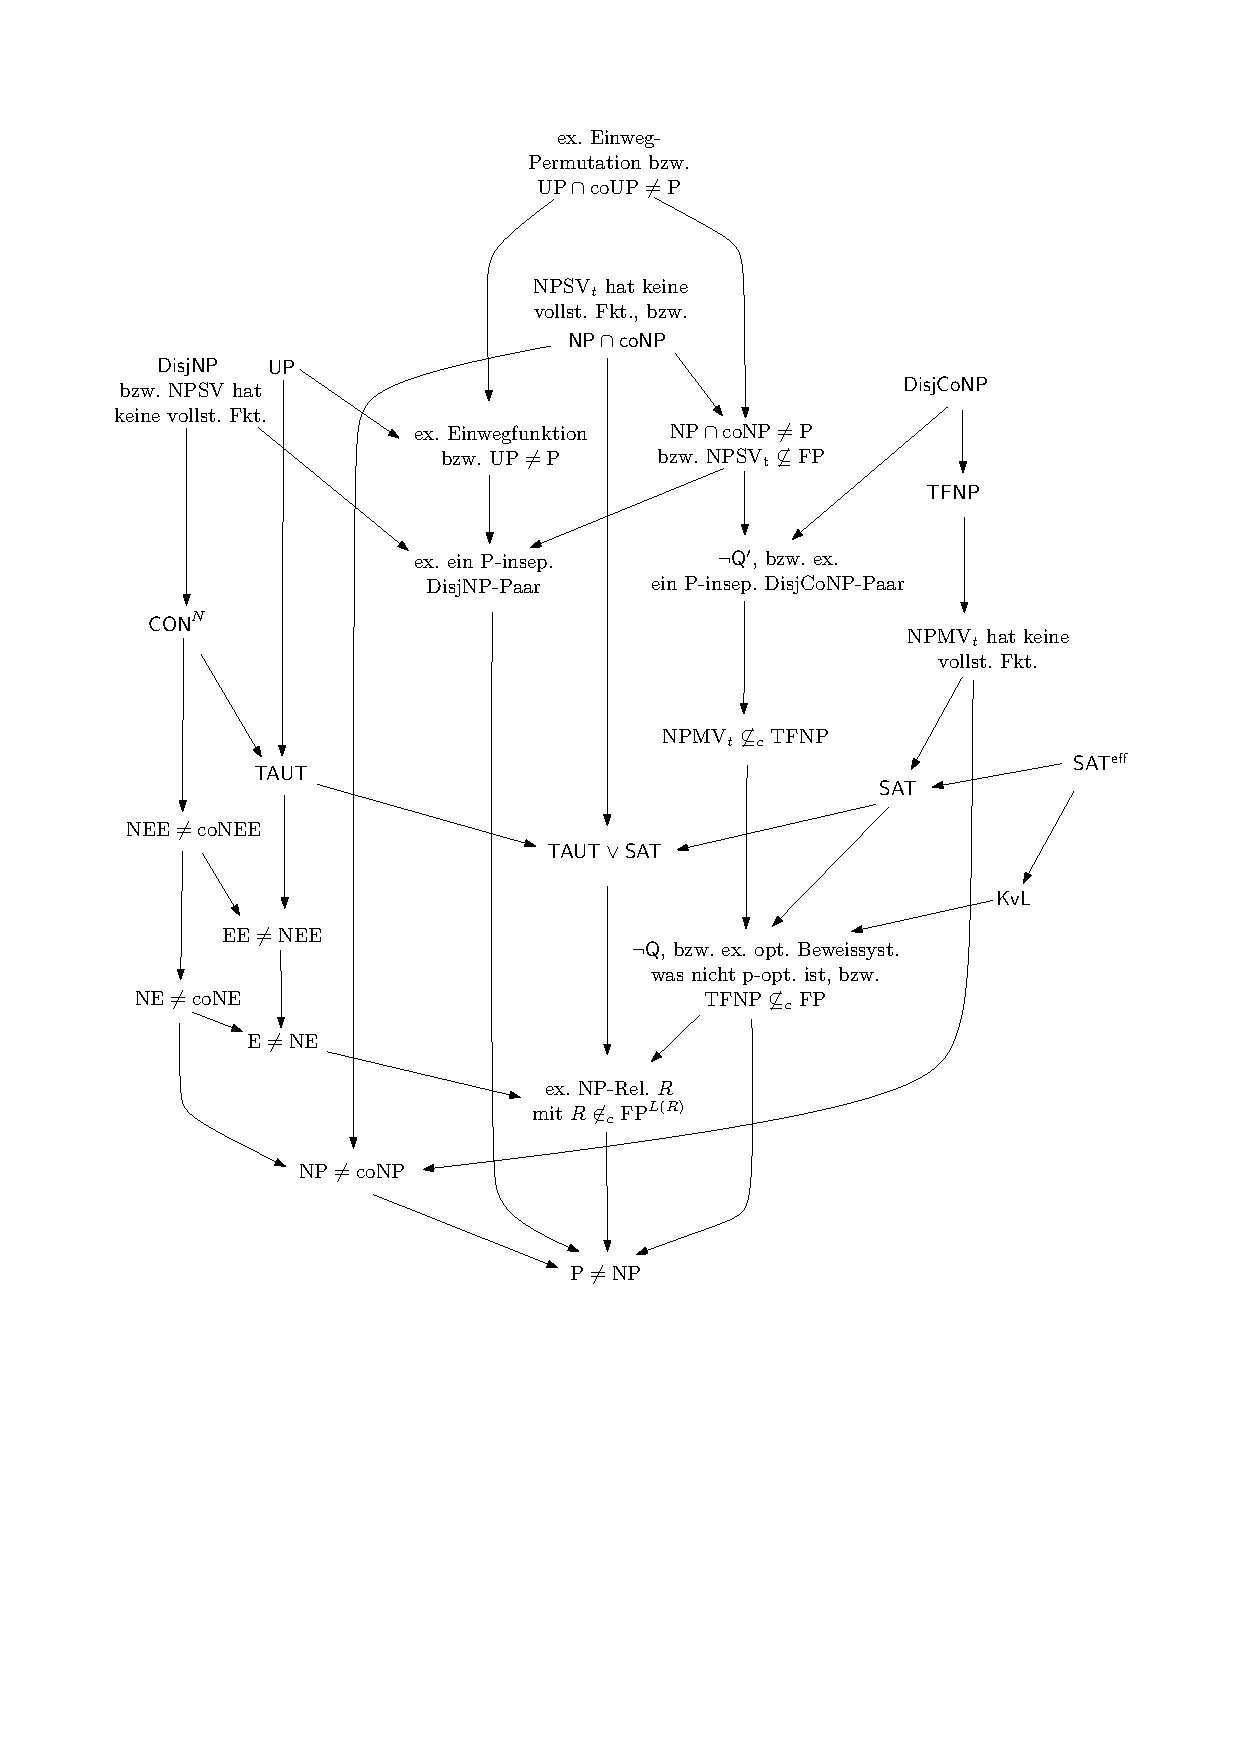
\includegraphics[page=1]{figures.pdf}
    \caption{Bekannte (relativierenden) Implikationen zwischen den betrachteten Hypothesen und weiteren Aussagen. Satz~\ref{thm:figure-implications} gibt Belegstellen für jede dieser Implikationen an.}\label{fig:figure-implications}
    \forcerectofloat
\end{figure*}

In anderen Worten sagt Satz~\ref{thm:q-fenner} aus, dass es unter Annahme von $\hQ$ modulo Umcodieren nur einen einzigen SAT-Solver gibt, und insbesondere alle SAT-Solver äquivalent zum trivialen Solver sind, welcher nur alle möglichen Belegungen ausprobiert.
Satz~\ref{thm:q-messner} macht eine analoge Aussage über Beweissysteme: egal wie komplex ein Beweissystem $h$ für $\mathtt{SAT}$ ist, wir können immer einen $h$-Beweis für $\phi$ in eine erfüllende Belegung für $\phi$ (quasi ein trivialer Beweis für $\phi\in\mathtt{SAT}$) transformieren. Damit ist auch leicht zu sehen, dass $\hQ\Rightarrow \neg\hSAT$, zumindest im unrelativierten Fall.

In Abschnitt~\ref{sec:q-vs-search} werden wir sehen, dass sich die obigen Charakterisierungen auf weitere (aber möglicherweise nicht alle) vollständigen NP-Relationen generalisiert, womit insbesondere auch die beiden Charakterisierungen von \citeauthor{fenner_inverting_2003} bzw. \citeauthor{kobler_is_2000} zu einer \emph{relativierbaren} Variante verallgemeinert werden.
Mit dieser Verallgemeinerung ist es dann auch für uns möglich, $\hQ$ formal in das Pudláksche Programm (u.a. durch $\hQ\Rightarrow \neg\hSAT$) einzuordnen. Hierfür führen wir jetzt schon den Begriff eines Standardbeweissystems bezüglich einer NP-Relation formal ein.

\begin{definition}[Standardbeweissystem einer NP-Relation]
    Sei $R$ eine NP-Relation. Wir definieren bezüglich $R$ das \emph{Standardbeweissystem} $\mathit{std}_R$ für $\Proj(R)$ wie folgt:
    \[ \mathit{std}_R(w) \defeq \begin{cases} x & \text{wenn $w=(x,y)$ und $(x,y)\in R$,}\\
    \bot & \text{sonst}.\end{cases} \qedhere \] 
\end{definition}
Damit ist, wie durch die Formulierung oben suggeriert, $\mathit{sat}=\mathit{std}_{\mathtt{rSAT}}$.
Insbesondere ist für jede NP-Relation $R$ das Standardbeweissystem $\mathit{std}_R$ für $\Proj(R)$ ehrlich, optimal, und hat kurze Beweise.
Beachte, dass sich aufgrund der speziellen Form der Beweise von Standardbeweissystemen die $\P$-Simulation knapper formulieren lässt:
\begin{observation}\label{obs:simulation-of-spps}
    Sei $R$ eine NP-Relation, und $h$ ein Beweissystem für $\Proj(R)$. Folgende Aussagen sind äquivalent:
    \begin{enumerate}
        \item $\mathit{std}_R$ $\P$-simuliert $h$.
        \item Es existiert Funktion $g\in\FP$, sodass
            \[ h(w)=x \implies \mathit{std}_R(x, g(w))=x \quad\text{(bzw. äquivalent $(x, g(w))\in R$)}. \]
    \end{enumerate}
\end{observation}
\begin{proof}
    \begin{prooflist}
    (1)$\implies$(2): Wenn $\mathit{std}_R$ das Beweissystem $h$ $\P$-simuliert, dann existiert eine Funktion $\pi\in\FP$ sodass $h(w)=x\rightarrow \mathit{std}_R(w)=x$ gilt.
    Haben wir also einen $h$-Beweis $w$ für $x$ gegeben, dann muss $\pi(w)$ von der Form $(x, z)$ mit $z\in\Sigma^*$ und $(x,z)\in R$ sein. Insbesondere können wir dann eine Funktion $g\in\FP$ angeben, sodass $g(w)$ die zweite Komponente von $\pi(w)$ ausgibt. Dann gilt $\mathit{std}_R(x, g(w))=x$.

    (2)$\implies$(1): Haben wir eine solche Funktion $g\in\FP$ gegeben, dann realisiert $\pi(w)=(h(w), g(w))$ die $\P$-Simulation bzw. Reduktion $h\leqmp \mathit{std}_R$.
    \end{prooflist}
\end{proof}

Bevor wir nun mit einer Diskussion zwischen Karp-Vollständigkeit und Levin-Vollständigkeit fortsetzen, machen wir folgende Beobachtung über $\hQ$ und der Ordnung der Simulation vs. $\P$-Simulation. Diese Beobachtung machen schon \textcite{kobler_is_2000}, aber deren Beweis (vgl. \cite[Thm.~5.2]{messner_simulation_2001}) relativiert insbesondere nicht. Wir zeigen die Aussage hier über eine nichttriviale Verallgemeinerung, welche insbesondere relativiert.
\begin{theorem}\label{thm:q-simulation}
    Folgende Aussagen sind äquivalent:
    \begin{enumerate}
        \item $\hQ$.
        \item Sei $L$ eine Menge und $h$, $g$ je Beweissysteme für $L$. Es gilt
            \[ \text{$h$ simuliert $g$} \iff \text{$h$ $\P$-simuliert $g$}. \]
        \item Für jedes Beweissystem $h$ gilt: $h$ ist optimal $\iff$ $h$ ist $\P$-optimal.
        \item Jedes ehrliche Beweissystem $h$ ist $\P$-optimal.
    \end{enumerate}
\end{theorem}
\begin{proof}
    \begin{prooflist}
    \item (1)$\implies$(2): Die Richtung von rechts nach links ist klar. Wir zeigen die andere Richtung. Nach Voraussetzung kann $h$ das Beweissystem $g$ simulieren, das heißt es existiert eine (nicht notwendigerweise effiziente) Funktion $\pi$ sodass $g(w)=h(\pi(w))$, und gleichzeitig ist $|\pi(w)|\leq q(|w|)$ für ein geeignetes Polynom $q$.

Betrachte folgende Multifunktion $f$:
\[ \fset{}f(w) \defeq  \{ y \mid \exists y\in\Sigma^{\leq q(|w|)}, g(w)=h(y) \}. \]
Es lässt sich leicht zeigen, dass $f\in\NPMV$, über einen geeigneten NPTM-Transduktor. 
Es ist sogar $f\in\NPMV_t$, denn für jedes $w\in\Sigma^*$ gilt mindestens $\pi(w)\in \fset{}f(w)$.

Mit $\hQ$ gilt nach Satz~\ref{thm:q-orig} also $f\in\NPMV_t\subseteqc \FP$, also existiert eine Funktion $f'\in\FP$ welche eine Verfeinerung von $f$ ist. Diese Funktion übersetzt $g$-Beweise $w$ für $x$ effizient in $h$-Beweise für $x$: 
Sei $g(w)=x$, dann gilt
\[ f'(w) = y \quad\text{mit } y\in\fset{}f(w), \text{ also gilt } y\in\Sigma^{\leq q(|w|)}, x=g(w)=h(y). \]
Damit ist $h(f'(w))=x$ bzw. $f'(w)$ ein $h$-Beweis für $x$, wie gewünscht.

\item (2)$\implies$(3): Klar.

\item (3)$\implies$(4): Klar, denn wenn $h$ ehrlich ist, dann hat es insbesondere auch kurze Beweise. Also ist $h$ auch optimal (Beobachtung~\ref{obs:super-ps-sind-opt}), und nach (3) dann auch $\P$-optimal.

\item (4)$\implies$(1): Wir zeigen, dass mit Voraussetzung (4) auch $\TFNP\subseteqc \FP$ gilt, was nach Satz~\ref{thm:q-orig} äquivalent zu $\hQ$ ist. Sei hierfür $R\in\TFNP$ gegeben.

    Das Standardbeweissystem $\mathit{std}_R$ für $\Sigma^*$ ist ehrlich, also nach (4) auch ein $\P$-optimales Beweissystem für $\Sigma^*$. Beachte, dass auch die Identitätsfunktion $\mathrm{id}$ ein Beweissystem für $\Sigma^*$ ist. Also kann $\mathit{std}_R$ das Beweissystem $\mathrm{id}$ $\P$-simulieren. Nach Beobachtung~\ref{obs:simulation-of-spps}(2) existiert also eine Funktion $g\in\FP$ sodass $\mathrm{id}(w)=x\rightarrow (x, g(w))\in R$. Da nun aber $\mathrm{id}(x)=x$ gilt $(x, g(x))\in R$, also ist $g$ eine Verfeinerung von $R$. Damit $R\inc\FP$, wie gewünscht.
    \end{prooflist}
\end{proof}

%Bevor wir nun mit einer Diskussion zwischen Karp-Vollständigkeit und Levin-Vollständigkeit fortsetzen, schließen wir diesen Einstieg mit folgender einfachen Beobachtung ab:
%\begin{observation}\label{obs:spps-honest}
    %Für jede NP-Relation $R$ ist das Standardbeweissystem $\mathit{std}_R$ für $\Proj(R)$ ehrlich, optimal, und hat kurze Beweise.
%\end{observation}
%\begin{proof}
    %Nachdem $R$ polynomiell längenbeschränkt ist, folgt sofort dass $\mathit{std}_R$ kurze Beweise hat. 
    %Nach Beobachtung \ref{obs:super-ps-sind-opt} damit auch optimal.
    %Insbesondere hat $\mathit{std}_R$ \emph{nur} polynomiell längere Beweise, also ist $\mathit{std}_R$ ehrlich.
%\end{proof}

\section{Karp-Vollständigkeit vs. Levin-Vollständigkeit}\label{sec:karp-vs-levin}

Wir wiederholen hier erneut die zentrale offene Frage und Vermutung aus Abschnitt~\ref{sec:levin}:

\begin{reptheorem}{Frage}{question:kvl}
    Sei $R$ eine NP-Relation.
Wenn $\Proj(R)$ eine $\leqmp$-vollständige Menge für $\NP$ ist, ist dann auch $R$ eine $\leqlp$-vollständige NP-Relation für $\FNP$?
\end{reptheorem}

\begin{reptheorem}{Vermutung}{conj:kvl}[$\mathsf{KvL}$]
    Es existiert eine NP-Relation $R$ sodass $\Proj(R)$ $\leqmp$-vollständig für $\NP$ ist, aber $R$ ist nicht $\leqlp$-vollständig für $\FNP$.
\end{reptheorem}

Zunächst sei hier noch einmal hervorgehoben, dass eine negative Beantwortung der Frage~\ref{question:kvl}, also ein Beweis von $\mathsf{KvL}$ schwer ist. Zum einen haben wir bereits gesehen, dass ein Beweis $\mathsf{KvL}$ auch sofort $\P\neq\NP$ beweisen würde. Insbesondere ist ein relativierender Beweis von $\mathsf{KvL}$ ausgeschlossen, denn existiert ein Orakel, relativ zu diesem $\neg\mathsf{KvL}$ (z.B. ein PSPACE-vollständiges Orakel, welches $\NP$ auf $\P$ kollabiert).
Auch für eine positive Beantwortung der Frage (also ein Beweis für $\neg\mathsf{KvL}$) fehlen uns konkrete Indizien.

Wir werden uns daher im Folgenden insbesondere auf Beziehungen zwischen $\mathsf{KvL}$ und gewissen anderen Hypothesen konzentrieren.
In diesem Sinne möchte ich argumentieren, dass die obige Frage bzw. Vermutung eng mit der Hypothese $\hQ$ zusammenhängt.
Im Speziellen werden wir sehen, dass die Hypothese $\hQ$ so charakterisiert werden kann, dass sie einer Verstärkung der Vermutung $\neg\mathsf{KvL}$ entspricht.\footnote{\textcite{fenner_inverting_2003} gaben hierbei eine ähnliche Aussage an (Cor.~3: „$\hQ$ holds iff every Karp reduction from $A$ to $B$ can be extended to a Levin reduction“), es ist aber hervorzuheben, dass die Autoren von einem unüblichen Begriff von Levin-Reduktionen ausgehen, der sich von dem hier verwendeten unterscheidet. Dieser umfasst nicht eine „Rückwärts-Translation“ von Zertifikaten für $B$-Instanzen zu $A$-Instanzen, sondern eine „Vorwärts-Translation“ von Zertifikaten für $A$-Instanzen zu $B$-Instanzen.}

\begin{theorem}\label{thm:q-as-levin}
    Folgende Aussagen sind äquivalent:
    \begin{enumerate}
        \item Hypothese $\hQ$.
        \item Für jedes Paar von NP-Relationen $A, B$ gilt:
            \[ \Proj(A) \leqmp \Proj(B) \iff A \leqlp B. \]
    \end{enumerate}
\end{theorem}
\begin{proof}
    \begin{prooflist}
\item (1)$\implies$(2): Die Richtung von rechts nach links ist klar. Für die andere Richtung sei $\Proj(A) \leqmp \Proj(B)$ mit $A,B$ NP-Relationen. Sei $q$ hierbei die Zertifikatsschranke von $A$.
    Wir wollen nun eine Levin-Reduktion von $A$ auf $B$ angeben. Sei $f\in \FP$ die Funktion, welche die Reduktion $\Proj(A) \leqmp \Proj(B)$ realisiert.
    Zunächst halten wir fest, dass unter (1) das Standardbeweissystem $\mathit{std}_R$ $\P$-optimal ist, denn es ist ehrlich, also nach Satz~\ref{thm:q-simulation} auch $\P$-optimal.

    Definiere folgendes Beweissystem
    \[ h(w) = \begin{cases} x & \text{falls $w=0\langle x, y\rangle$ und $(x,y)\in A$} \\ x & \text{falls $w=1\langle x, z\rangle$ und $(f(x), z)\in B$} \\ \bot & \text{sonst}. \end{cases}\]
    Es ist leicht zu sehen, dass $h$ ein Beweissystem für $\Proj(A)$ ist.
    Also kann $\mathit{std}_R$ das Beweissystem $h$ $\P$-simulieren. Mit Beobachtung~\ref{obs:simulation-of-spps} folgt, dass eine Funktion $g$ existiert mit
    \[ h(w)=x\implies (x, g(w))\in A. \]
    Wir zeigen nun, dass $A\leqlp B$. Sei hierfür $f$ von oben die entsprechende Reduktionsfunktion.
    Es gilt
    \begin{gather*}
        (f(x), z)\in B \implies h(1\langle x, z\rangle)=x \implies (x, \underbrace{g(1\langle x, z\rangle)}_{g'(x, z)})\in A,
    \end{gather*}
    heißt mit der Translationsfunktion $g'\in\FP, g'(x,z)=g(1\langle x,z\rangle)$ können wir $B$-Zertifikate für $f(x)$ in $A$-Zertifikate für $x$ umrechnen, wie gewünscht.

\item (2)$\implies$(1): Wir zeigen $\TFNP\subseteqc \FP$; das ist nach Satz~\ref{thm:q-orig} äquivalent zu (1). Sei nun $A$ eine totale NP-Relation
    Definiere nun die NP-Relation
    \[ B \defeq \{ (x, \epsilon) \mid x\in\Sigma^* \}. \]
    Es ist leicht zu sehen das $\Proj(A)=\Sigma^*=\Proj(B)$ und dass $\Proj(A)\leqmp\Proj(B)$ über die Identitätsfunktion.
    Nach Annahme (2) lässt sich nun diese Reduktion zu einer Levin-Reduktion $A\leqlp B$ verstärken, mit Reduktionsfunktion $f\in\FP$ und  Translationsfunktion $g\in\FP$.

    Sei nun ein Wort $x\in\Sigma^*$ gegeben. Hieraus können wir effizient ein $A$-Zertifikat berechnen: es gilt $(f(x),\epsilon)\in B$, also auch $(x, g(x, \epsilon))\in A$. Heißt, $g(x, \epsilon)$ ist unser gesuchtes $A$-Zertifikat, welches wir auch effizient berechnen können.
\end{prooflist}
\end{proof}

Beachte, dass in Aussage (2) die Implikation von rechts nach links ohnehin immer gilt. 
Damit lässt sich Aussage (2) auch so formulieren, dass jede Karp-Reduktion zu einer Levin-Reduktion verstärkt werden kann, indem zur Reduktionsfunktion $f$ eine geeignete Translationsfunktion $g$ hinzugefügt wird.
Mit dieser Charakterisierung folgt auch unmittelbar, dass $\hQ$ hinreichend für $\neg\mathsf{KvL}$ ist: ist $\Proj(A)$ $\leqmp$-vollständig, dann lässt sich jede Reduktion $\Proj(B)\leqmp \Proj(A)$ zu einer $\leqlp$-Reduktion $B\leqlp A$ verstärken; also ist $A$ $\leqlp$-vollständig.


\begin{corollary}\label{cor:kvl-implies-q}
    $\hQ\implies \neg\mathsf{KvL}$.
\end{corollary}
%\begin{proof}
    %Wir starten mit der Voraussetzung $\hQ$.
    %Wir wollen nun $\neg\mathsf{KvL}$ zeigen. Sei hierfür $R$ eine beliebige NP-Relation sodass $\Proj(R)$ $\leqmp$-vollständig für $\NP$ ist.
    %Damit gilt also schon für alle weiteren NP-Relationen $A$, dass $\Proj(A)\leqmp\Proj(R)$.
    %Nach Satz~\ref{thm:q-as-levin} gilt nun $A\leqlp R$. Also ist $R$ auch $\leqlp$-vollständig für $\FNP$, wie gewünscht und wir haben $\neg\mathsf{KvL}$ gezeigt.
%\end{proof}

\subsection*{P-Quasi-Simulation}

Was sind natürliche notwendige Bedingungen für die Hypothese $\mathsf{KvL}$? Diese Frage erscheint tatsächlich wesentlich schwieriger als gedacht. Insbesondere scheint es unklar, ob aus irgend einer von Pudláks Hypothesen die Aussage $\mathsf{KvL}$ folgt.

Um uns dieser Frage dennoch zu nähern, beginnen wir zunächst, die Hypothese $\mathsf{KvL}$ auf weitere Weisen zu charakterisieren. Es ist intuitiv ersichtlich, dass für eine feste Sprache $L$ die NP-Relationen für $L$, die ehrlichen Beweissysteme für $L$, und die NPTMs, welche $L$ entscheiden, alle im breitesten Sinn „Zertifikatsschemata“ sind, und alle diese Berechnungsmodelle untereinander umgeschrieben werden können: jede NP-Relation $R$ induziert ein ehrliches Beweissystem $\mathit{std}_R$, jedes ehrliche Beweissystem $h$ induziert eine NPTM $N$ mit $L(N)=L$ (rate einen $h$-Beweis polynomieller Länge), und jede NPTM $N$ mit $L(N)=L$ induziert eine NP-Relation für $L$ ($w$ ist eine Lösung für $x$ wenn $w$ ein akzeptierender Rechenweg auf $N(x)$ ist). Insbesondere ist für ein ehrliches Beweissystem $h$ die Umkehrrelation $h^{-1}=\{(x,w) \mid h(w)=x \} $ eine NP-Relation für $\img(h)$.

Wir wollen nun die existierende $\leqlp$-Ordnung auf den NP-Relationen aufgreifen, und diese auf die ehrlichen Beweissysteme übertragen. Wir definieren hierfür eine abgeschwächte Variante der $\P$-Simulation, welche der $\leqlp$-Reduktion nachempfunden ist.
\begin{definition}
    Seien $h,h'$ Beweissysteme für $L$. Das Beweissystem $h$ \emph{$\P$-quasi-simuliert} $h'$ falls Funktionen $f,g\in\FP$ existieren sodass
    \begin{enumerate}
        \item $x\in L \iff f(x)\in L$,
        \item $ h'(w)=f(x) \implies h(g(x, w)) = x. $\qedhere
    \end{enumerate}
    %Kann das Beweissystem $h$ jedes Beweissystem $h'$ für $L$ effektiv $\P$-simulieren, dann ist $h$ \emph{effektiv $\P$-optimal}.
\end{definition}
In anderen Worten, falls $h$ das Beweissystem $h'$ $\P$-quasi-simuliert, dann kann $h$ zwar nicht \emph{jeden} $h'$-Beweis $w$ für $x\in L$ in einen $h$-Beweis für (das gleiche) $x$ effizient umrechnen, es kann aber zumindest alle \emph{relevanten} $h'$-Beweise effizient umrechnen, nämlich für jedes $x\in L$ die $h'$-Beweise für $f(x)$ in $h$-Beweise für $x$.
%Anstelle „$h$ $\P$-simuliert effektiv $h'$“ ließe sich äquivalent auch $h^{-1}\leqlp h'^{-1}$ schreiben. Beachte, dass die Relation $h^{-1}$ nur Lösungen mit ihren Beweisen reliert.
Die $\P$-Quasi-Simulation ist reflexiv und transitiv, und sie 
liegt insbesondere zwischen Simulation und $\P$-Simulation: $\P$-Simulation impliziert $\P$-Quasi-Simulation impliziert Simulation.
Ferner ist diese Art von Simulation \emph{effektiv}, in dem Sinn dass die $\P$-invertierbaren Beweissysteme selbst unter $\P$-Quasi-Simulation abgeschlossen sind.

Es ist intuitiv ersichtlich, dass $\P$-quasi-Simulation auf ehrlichen Beweissystemen das Analog der $\leqlp$-Reduktion auf NP-Relationen darstellt. Wir können folgende Beobachtung festhalten:
\begin{observation}\label{obs:p-quasi-sim-vs-leqlp}
    Sei $L\in\NP$, seien $h, h'$ zwei ehrliche Beweissysteme für $L$, und seien $R, R'$ zwei NP-Relationen für $L$.
    \begin{enumerate}
        \item $h^{-1}\leqlp h'^{-1} \iff \text{$h$ kann $h'$ $\P$-quasi-simulieren.}$
        \item $R\leqlp R' \iff \text{$\mathit{std}_R$ kann $\mathit{std}_{R'}$ $\P$-quasi-simulieren.}$
    \end{enumerate}
\end{observation}
\begin{proof}
    \begin{prooflist}
    \item Zu (1): Wir haben
        \begin{gather*}
            h^{-1}\leqlp h'^{-1} \iff \exists f,g\in\FP.\, [(f(x), w)\in h'^{-1} \rightarrow (x, g(x, w))\in h^{-1}]\\
            \iff \exists f,g\in\FP.\, [h'(w)=f(x) \rightarrow h(g(x, w))=x]\\
            \iff \text{$h$ kann $h'$ $\P$-quasi-simulieren,}
        \end{gather*}
        wobei hier die existenziell quantifizierte Variable $f$ nur über Reduktionsfunktionen von $L$ auf $L$ reichen soll.
    \item Zu (2): Ähnlich wie (1), nur etwas aufwändiger. Wir haben
        \begin{gather*}
            R\leqlp R' \iff \exists f,g\in\FP.\, [(f(x), w)\in R' \rightarrow (x, g(x, w))\in R]\\
            \iff \exists f,g\in\FP.\, [\mathit{std}_{R'}(f(x), w)=f(x) \rightarrow \mathit{std}_R(x, g(x, w))=x\\
            \iff \exists f,g'\in\FP.\, [\mathit{std}_{R'}(w')=f(x) \rightarrow \mathit{std}_R(g'(x, w'))=x\\
            \iff \text{$\mathit{std}_{R}$ kann $\mathit{std}_{R'}$ $\P$-quasi-simulieren,}
        \end{gather*}
        wobei wieder die existenziell quantifizierte Variable $f$ nur über Reduktionsfunktionen von $L$ auf $L$ reichen soll.
    \end{prooflist}
\end{proof}

Die intuitive Aussage von $\neg\mathsf{KvL}$ „Alle NP-Relationen für NP-vollständige Sprache $L$ sind im Wesentlichen gleich“ überträgt sich nun auch auf ehrliche Beweissysteme:
\begin{theorem}\label{thm:kvl-ps}
    Folgende Aussagen sind äquivalent:
    \begin{enumerate}
        \item Aussage $\neg\mathsf{KvL}$.
        \item Für jede $\leqmp$-vollständige Menge $L\in\NP$ gilt: Wenn $R, R'$ zwei NP-Relationen für $L$ sind, dann
            \[ R \leqlp R'. \]
        \item Für jede $\leqmp$-vollständige Menge $L\in\NP$ gilt: Wenn $h, h'$ zwei ehrliche Beweissysteme für $L$ sind, dann
            \[  \text{$h$ $\P$-quasi-simuliert $h'$}. \]
        \item Für eine $\leqlp$-vollständige NP-Relation $R$ gilt: Wenn $R'$ eine NP-Relation für $\Proj(R)$ ist, dann
            \[ R \leqlp R'. \]
    \end{enumerate}
\end{theorem}
\begin{proof}
    \begin{prooflist}
        \item (1)$\implies$(2): Klar, denn mit (1) ist $R'$ $\leqlp$-vollständig.
        \item (2)$\implies$(4): Klar, ist ja $\mathtt{rSAT}$ $\leqlp$-vollständig.
        \item (4)$\implies$(1): Sei $Q$ eine NP-Relation, wobei $\Proj(Q)$ $\leqmp$-vollständig für $\NP$ ist. Wir werden zeigen, dass $R\leqlp Q$, wobei dann auch $Q$ $\leqlp$-vollständig ist (Beob.~\ref{lemma:fnp-completeness}), wie gewünscht.
        Die Argumentation verläuft hierbei ähnlich wie bei Satz~\ref{thm:q-as-levin}. Sei $f\in\FP$ die Funktion, welche $\Proj(R)\leqmp \Proj(Q)$ realisiert.
        Sei nun
        \[ R' = \{ (x, 0y) \mid (x,y)\in R \} \cup \{ (x, 1z) \mid (f(x), z)\in Q \}. \]
        Es lässt sich leicht zeigen, dass $R'$ eine NP-Relation für $\Proj(R)$ ist.
        Nach (4) gilt nun $R \leqlp R'$. Ebenso gilt $R'\leqlp Q$, denn wir haben
\[ (f(x), z)\in Q \implies (x, \underbrace{1z}_{\mathclap{g(x,z)}})\in R', \]
        also realisiert $f$ als Reduktionsfunktion und $g(x,z)\defeq 1z$ als Translationsfunktion die Levin-Reduktion $R'\leqlp Q$. Damit gilt $R\leqlp R'\leqlp Q$ wie gewünscht.
        \item (2)$\iff$(3): Einfach mit Beobachtung~\ref{obs:p-quasi-sim-vs-leqlp} nachweisbar.
    \end{prooflist}
\end{proof}

Als Korollar erhalten wir dabei insbesondere folgende Aussage, welche $\mathsf{KvL}$ mit Standardbeweissystemen von $\leqlp$-vollständigen NP-Relationen in Beziehung setzt:
\begin{corollary}\label{cor:kvl-spps}
    Sei $R$ eine NP-Relation, sodass $R$ $\leqlp$-vollständig ist.
    Folgende Aussagen sind äquivalent:
    \begin{enumerate}
        \item Aussage $\neg\mathsf{KvL}$.
        \item Für alle ehrlichen Beweissysteme $h$ mit $\img(h)=\Proj(R)$ gilt
        \[  \text{$\mathit{std}_R$ $\P$-quasi-simuliert $h$}. \]
    \end{enumerate}
\end{corollary}
\begin{proof}
    \begin{prooflist}
    \item (1)$\implies$(2): Klar, denn $\mathit{std}_R$ ist ehrlich, und mit Satz~\ref{thm:kvl-ps}(3) kann $\mathit{std}_R$ damit $h$ auch $\P$-quasi-simulieren.

    \item (2)$\implies$(1): Wir zeigen die Aussage von Satz~\ref{thm:kvl-ps}(4), womit auch $\neg\mathsf{KvL}$ bzw (1) gilt. Sei hierfür $R'$ eine NP-Relation für $\Proj(R)$. Mit (2) wissen wir dass $\mathit{std}_R$ das Beweissystem $\mathit{std}_{R'}$ $\P$-quasi-simulieren kann. Mit Beobachtung~\ref{obs:p-quasi-sim-vs-leqlp}(2) folgt $R\leqlp R'$.
    \end{prooflist}
\end{proof}

Unter dieser Charakterisierung erhalten wir einen zweiten trivialen Beweis von Korollar~\ref{cor:kvl-implies-q}: $\hQ$ ist hinreichend für $\neg\mathsf{KvL}$, denn unter Annahme von $\hQ$ ist jedes ehrliche Beweissystem $\P$-optimal, heißt auch das Standardbeweissystem $\mathit{std}_{\mathtt{rKAN}}$ für $\mathtt{KAN}$ ist $\P$-optimal (Satz~\ref{thm:q-simulation}), kann also insbesondere auch alle ehrlichen Beweissysteme $h$ $\P$-quasi-simulieren. Damit auch $\neg\mathsf{KvL}$ (Korollar~\ref{cor:kvl-spps}).

Mittels unserem Begriff der $\P$-Quasi-Simulation können wir nun auch die Hypothese $\hSAT$ auf natürliche Weise verstärken:
\begin{conjecture}[$\mathsf{SAT^{q}}$]
    Es existiert keine $\leqmp$-vollständige Menge $L$ für $\NP$ mit einem Beweissystem $h$, welches alle anderen ehrlichen Beweissysteme für $L$ $\P$-quasi-simulieren kann. 
\end{conjecture}
Diese Verstärkung ist am sichtbarsten, wenn wir uns überlegen, wie die Negation $\neg\hSAT$ zu $\neg\mathsf{SAT^{q}}$ in zwei Aspekten abgeschwächt wird.
Erstens der Umfang: es wird nicht mehr verlangt, dass ein Beweissystem $h$ existiert, welche \emph{alle} Beweissysteme $\P$-simulieren kann, sondern nur noch alle \emph{ehrlichen} Beweissysteme.
Zweitens die Beziehung: es wird nicht mehr $\P$-Simulation, sondern nur noch $\P$-\emph{Quasi}-Simulation vorausgesetzt.

Wir sehen nun, dass $\mathsf{SAT^{q}}$ eine Verstärkung von sowohl $\hSAT$ als auch $\mathsf{KvL}$ ist:
\begin{corollary}\label{cor:sateff-generalizes-sat}
    \begin{enumerate}
        \item $\mathsf{SAT^{q}}\implies \hSAT$
        \item $\mathsf{SAT^{q}}\implies \mathsf{KvL}$
    \end{enumerate}
\end{corollary}
\begin{proof}
    Für (1) haben wir bereits argumentiert. Wir zeigen nur noch (2) mittels Kontraposition. Unter $\neg\mathsf{KvL}$ folgt mit der Formulierung aus Korollar~\ref{cor:kvl-spps}(2), dass das Standardbeweissystem der $\leqlp$-vollständigen NP-Relation $\mathtt{rSAT}$ alle ehrlichen Beweissysteme $\P$-quasi-simulieren kann. Also hat die Menge $\mathtt{KAN}$ \emph{ein} Beweissystem, welches alle ehrlichen Beweissysteme $\P$-quasi-simulieren kann.
\end{proof}

Wir haben damit also je eine notwendige ($\neg\hQ$) und eine hinreichende Hypothese ($\mathsf{SAT^{q}}$) für $\mathsf{KvL}$. Durch die Charakterisierung von $\neg\mathsf{KvL}$ über Beweissysteme ergibt sich durch Korollar~\ref{cor:kvl-spps} eine interessante Ähnlichkeit zur Hypothese $\hQ$. Wir wollen diese beiden Hypothesen im Folgenden kurz gegenüberstellen.
Zur Anschaulichkeit beziehe ich mich hierbei auf die NP-Relation $\mathtt{rSAT}$. (Durch Ergebnisse im nächsten Abschnitt wird klar, dass sich dieses Argument auch auf $\mathtt{rKAN}$ relativierend überträgt.)
Wir haben
\begin{itemize}[midpenalty=10000]
    \item $\hQ$ genau dann wenn $\mathit{sat}$ jedes ehrliche Beweissystem $\P$-simulieren kann (Satz~\ref{thm:q-fenner}),\sidenote{Satz~\ref{thm:q-fenner} macht zwar nur Aussagen über NPTMs, aber es ist leicht zu sehen, dass diese mit den ehrlichen Beweissystemen identifiziert werden können. Vgl. auch Satz~\ref{thm:q-fenner-generalized}.}
    \item $\neg\mathsf{KvL}$ genau dann wenn $\mathit{sat}$ jedes ehrliche Beweissystem $\P$-quasi-simulieren kann (Korollar~\ref{cor:kvl-spps}).
\end{itemize}
Damit wird deutlich, dass die die Hypothesen $\hQ$ und $\neg\mathsf{KvL}$ äquivalent sind, falls die $\P$-Quasi-Simulation genauso stark ist wie die $\P$-Simulation.

%Insbesondere vermute ich, dass möglicherweise sogar $\hQ\Leftrightarrow\neg\mathsf{KvL}$ gelten könnte. Die Richtung von links nach rechts haben wir bereits in Korollar~\ref{cor:kvl-implies-q} gesehen, und ist ferner in der hier genannten Charakterisierung trivial. Für die Richtung von rechts nach links möchte ich nun plausibilisieren, dass $\neg\mathsf{KvL}\land\neg\hQ$ zu einem Widerspruch führt.

%Unter Annahme von $\neg\hQ$ folgt nach Satz~\ref{thm:q-fenner}, dass das Standardbeweissystem $\mathit{sat}$ von $\mathtt{rSAT}$ ein bestimmtes ehrliches Beweissystem $h$ nicht $\P$-simulieren kann.
%Wir haben also für alle Funktionen $f\in\FP$ 
%\begin{equation} h(w)=\psi \rlap{\hspace*{2pt}\raisebox{2.3pt}{$\quad\not$}}\implies  \text{$f(w)$ erfüllt $\psi$}.\label{eq:weak-irreducibility} \end{equation}
%In anderen Worten: obwohl wir einen $h$-Beweis $w$ für die Erfüllbarkeit der Formel $\phi$ haben, können wir nicht effizient eine erfüllende Belegung aus $w$ berechnen.

%Nun gilt aber nach Annahme auch $\neg\mathsf{KvL}$. Über Satz~\ref{thm:kvl-ps}(4) gilt, dass $\mathit{sat}$ das ehrliche Beweissystem $h$ $\P$-quasi-simulieren kann. Wir haben also zwei Funktionen $f', g'\in\FP$ sodass
%\begin{equation}\label{eq:effective-simulation} h(w)=f'(\phi) \implies \text{$g'(\phi, w)$ erfüllt $\phi$}. \end{equation}
%Beachte, dass die Funktion $f'$ notwendigerweise ungleich $\mathrm{id}$ ist. Wir können $f'$ so verstehen, dass diese $\phi$ gewissermaßen in eine einfachere Form bringt, für welche $h$-Beweise effizient verarbeitet werden können.

%Es ist also einerseits nicht möglich, aus dem $h$-Beweis $w$ effizient eine akzeptierende Belegung für $f(\phi)$ zu bestimmen, obwohl $w$ bezeugt dass $f(\phi)$ erfüllbar ist. (Ersetze in \eqref{eq:weak-irreducibility} $\psi$ mit $f(\phi)$.)
%Andererseits reicht der $h$-Beweis $w$ für $f(\phi)$ aber aus, um (zusammen mit der Information $\phi$) effizient wieder eine erfüllende Belegung für $\phi$ zu berechnen. 
%Diese Argumentation \emph{plausibilisiert} zwar einen Widerspruch, bzw. dass $\neg\hQ\land\neg\mathsf{KvL}$ wahrscheinlich falsch ist, ist aber natürlich kein solcher. Die Umkehrung von Korollar~\ref{cor:kvl-implies-q} bleibt offen.

Dennoch bleiben weitere Fragen offen, die wir hier aus Platzgründen nicht weiter verfolgen werden. 
Zum einen zur Charakterisierung von $\mathsf{KvL}$:
Wir konnten zwar $\mathsf{KvL}$ unter anderem als Aussage über Beweissysteme formulieren, aber sind auch noch weitere äquivalente Charakterisierungen möglich, z.B. ähnlich wie bei $\hQ$?

Zum anderen die Beziehungen zwischen $\mathsf{KvL}$ und anderen Hypothesen bzw. Annahmen.
Gibt es natürliche (z.B. kryptographische) Annahmen, welche hinreichend für $\mathsf{KvL}$ sind? Wie ist die Beziehung zu den anderen Pudlákschen Hypothesen? Wie verhält sich insbesondere $\hSAT$ zu $\mathsf{SAT^{q}}$? 
Diese Fragen werden wir zum Teil in Kapitel~\ref{chap:orakel} klären; dort wird ein Orakel konstruiert, welches zeigt, dass selbst unter der Annahme von $\hDisjNP\land\hUP$ es nicht möglich ist, mit relativierenden Beweismethoden auf $\mathsf{KvL}$ zu schließen.
Wir kommen hierauf am Ende dieses Kapitels noch einmal zurück.

Insgesamt ist durch die vorherigen Überlegungen aber ein erster Schritt getan, die Beziehung zwischen Levin- und Many-one-Vollständigkeit über die Vermutung $\mathsf{KvL}$ im Kontext des Pudlákschen Programms einzuordnen.
Weitere Forschung in diese Richtung erscheint vielversprechend.

\section{Hypothese $\hQ$ und Suchprobleme}\label{sec:q-vs-search}

Wie im Einstieg des Kapitels angesprochen, geben \textcite{fenner_inverting_2003} bzw. \textcite{kobler_is_2000} äquivalente Charakterisierungen der Hypothese $\hQ$ an, welche sich im Wesentlichen auf auf der $\leqlp$-Vollständigkeit von $\mathtt{rSAT}$ aufbauen (Satz~\ref{thm:q-fenner} und \ref{thm:q-messner}).
Wir wiederholen hier noch einmal die Aussagen, aber mit einer etwas abstrakteren Notation.
Wie schon angesprochen, können für eine feste Menge $L$ die ehrlichen Beweissysteme für $L$ mit den NPTMs identifiziert werden, welche $L$ entscheiden.
So können wir die anfangs genannten Charakterisierung von \citeauthor{fenner_inverting_2003} stattdessen folgendermaßen notieren:
\begin{reptheorem}{Satz}{thm:q-fenner}[\cite{fenner_inverting_2003}]
    Es gilt $\hQ$ genau dann wenn $h\leqmp\mathit{sat}$ für jedes ehrliche Beweissystem $h$ für $\mathtt{SAT}$. 
\end{reptheorem}
Die Charakterisierung von \citeauthor{kobler_is_2000} können wir auf ähnliche Weise über Standardbeweissysteme von NP-Relationen schreiben.
\begin{reptheorem}{Satz}{thm:q-messner}[\cite{kobler_is_2000}]
    Es gilt $\hQ$ genau dann wenn das Standardbeweissystem $\mathit{std}_\mathtt{rSAT}$ $\P$-optimal ist.
\end{reptheorem}

Diese beiden Charakterisierungen wollen wir im Folgenden verallgemeinern und von $\mathtt{rSAT}$ auf beliebige $\leqlp$-vollständige NP-Relationen $R$ übertragen. 
Hieraus ergibt sich schon unmittelbar der technische Beitrag, dass dann diese Charakterisierungen auch in einer relativierten Umgebung angewendet werden können, um z.B. ein geeignetes Orakel zu konstruieren, was $\hQ$ von anderen Hypothesen trennt.

Das ist für den zweiten Satz~\ref{thm:q-messner} ohne weitere zusätzliche Bedingungen möglich. Beachte, dass sich der hier präsentierte Beweis maßgeblich von dem ursprünglichen Beweis von \textcite[vgl.][Thm.~5.2]{messner_simulation_2001} unterscheidet, und insbesondere ohne sein (nichtrelativierendes) Padding-Argument auskommt.
\begin{theorem}\label{thm:q-messner-generalized}
    Sei $R$ eine beliebige $\leqlp$-vollständige NP-Relation.
    Folgende Aussagen sind äquivalent:
    \begin{enumerate}
        \item Aussage $\hQ$.
        \item Das Standardbeweissystem $\mathit{std}_R$ ist $\P$-optimal.
    \end{enumerate}
\end{theorem}
\begin{proof}
    \begin{prooflist}
    \item (1)$\implies$(2): 
        Das Standardbeweissystem $\mathit{std}_R$ ist ehrlich. Nach Satz~\ref{thm:q-simulation} ist $\mathit{std}_R$ damit $\P$-optimal.

    \item (2)$\implies$(1): Wir zeigen die Aussage, dass $\TFNP\subseteqc\FP$.  Nach Satz~\ref{thm:q-orig} ist das äquivalent zu $\hQ$. Sei hierfür ein solches $Q\in\TFNP$ gegeben

    Nachdem $R$ $\leqlp$-vollständig ist, haben wir Funktionen $f,g\in\FP$ mit
    \[ x\in \Proj(Q)\iff  f(x)\in\Proj(R), \quad (f(x), z)\in R\implies (x,g(x,z))\in Q. \]
    Definiere nun
    \[ h(w) = \begin{cases} f(x) & \text{wenn $w=0x$}\\ x & \text{wenn $w=1\langle x, y\rangle$ und $(x,y)\in R$} \\  \bot & \text{sonst} \end{cases}.\]
    Es ist leicht zu sehen, dass $h$ ein Beweissystem für $\Proj(R)$ ist, denn insbesondere gilt $f(x)\in\Proj(R)$ für jedes $x\in\Sigma^*$.
    Nach (2) gilt also $h\leqmp \mathit{std}_R$. Mit Beobachtung~\ref{obs:simulation-of-spps} haben wir eine Funktion $r\in\FP$, sodass
    \[ h(w)=x \implies (x, r(w))\in R. \]
    Damit gilt insbesondere
    \[ h(0x)=f(x)\implies (f(x), r(0x))\in R \implies (x, \underbrace{g(r(0x))}_{q(x)})\in Q. \]
    Damit ist $q(x) = g(r(0x))$, $q\in\FP$ eine Verfeinerung von $Q$, wie gewünscht.
\end{prooflist}
\end{proof}


Die andere Charakterisierung von \citeauthor{fenner_inverting_2003} ist umfangreicher.
Zunächst ist klar, dass „$h\leqmp\mathit{std}_R$ für alle ehrlichen Beweissysteme“ schwächer ist als „$h\leqmp\mathit{std}_R$ für alle Beweissysteme“, was ja nach vorigem Satz äquivalent zu $\hQ$ ist.
Tatsächlich gilt die Umkehrung scheinbar nicht für alle $\leqlp$-vollständigen NP-Relationen $R$. 
Die Autoren zeigen diese Umkehrung für die NP-Relation $\mathtt{rSAT}$, und nutzen hierbei die Eigenschaft aus, dass die entsprechenden Reduktionsfunktionen alle $\P$-invertierbar sind, bzw. in anderen Worten, die $\leq_\mathrm{L,1,i}^\mathrm p$-Vollständigkeit von $\mathtt{rSAT}$.

Wir werden im Folgenden diese Voraussetzung abschwächen, und betrachten dabei folgende Verstärkung der $\leqmp$-Reduktion.
\begin{definition}[Ehrliche Levin-Reduzierbarkeit]
    Seien $Q, R$ zwei NP-Relationen. Wir sagen dass \emph{$Q$ sich auf $R$ ehrlich Levin-reduzieren lässt}, bzw. $Q\leq_\mathrm{L,h}^\mathrm p R$ wenn $Q\leqlp R$, und die zugehörige Reduktionsfunktion $f$ ehrlich ist.

    Definiere $\leq_\mathrm{L,h}^\mathrm p$-Vollständigkeit entsprechend.
\end{definition}
Beachte, dass $\leq_\mathrm{L,h}^\mathrm p$ zwischen $\leqlp$ und $\leq_\mathrm{L,1,i}^\mathrm{p}$ liegt:
\[ Q\leq_\mathrm{L,1,i}^\mathrm{p} R \implies Q\leq_\mathrm{L,h}^\mathrm p R \implies Q\leqlp R. \]
Damit impliziert $\leq_\mathrm{L,1,i}^\mathrm{p}$-Vollständigkeit eine  $\leq_\mathrm{L,h}^\mathrm p$-Vollständigkeit, und diese eine $\leqlp$-Vollständigkeit.

Mit dem Begriff der ehrlichen Reduzierarkeit können wir den vorigen Beweis von Satz~\ref{thm:q-messner-generalized} erweitern, womit wir Satz~\ref{thm:q-fenner} generalisieren und relativieren. 
\begin{theorem}\label{thm:q-fenner-generalized}
    Sei $R$ eine beliebige $\leq_\mathrm{L,h}^\mathrm p$-vollständige NP-Relation.
    Folgende Aussagen sind äquivalent:
    \begin{enumerate}
        \item Aussage $\hQ$.
        \item Das Standardbeweissystem $\mathit{std}_R$ ist $\P$-optimal.
        \item Für jedes ehrliche Beweissystem $h$ für $\Proj(R)$ gilt $h\leqmp \mathit{std}_R$.
    \end{enumerate}
\end{theorem}
\begin{proof}
    \begin{prooflist}
    \item (1)$\implies$(2): Klar, nach Satz~\ref{thm:q-simulation} ist mit (1) das Beweissystem $\mathit{std}_R$ $\P$-optimal.

        \item (2)$\implies$(3): Klar.

        \item (3)$\implies$(1): Analog wie bei Satz~\ref{thm:q-messner-generalized}.
            Wir zeigen wieder die Aussage, dass $\TFNP\subseteqc\FP$. Sei hierfür ein solches $Q\in\TFNP$ gegeben.
    Nachdem $R$ $\leqlp$-vollständig ist, haben wir Funktionen $f,g\in\FP$, welche $Q\leqlp R$ realisieren.
    %\[ x\in \Proj(Q)=\Sigma^*\implies  f(x)\in\Proj(R), \quad (f(x), z)\in R\implies (x,g(x,z))\in Q. \]
    Definiere nun
    \[ h(w) = \begin{cases} f(x) & \text{wenn $w=0x$}\\ x & \text{wenn $w=1\langle x, y\rangle$ und $(x,y)\in R$} \\  \bot & \text{sonst} \end{cases}.\]
    Es ist leicht zu sehen, dass $h$ ein Beweissystem für $\Proj(R)$ ist.
    Insbesondere ist $h$ ehrlich, denn $f$ ist ehrlich.
    Damit gilt mit (3), dass $h\leqmp \mathit{std}_R$; mit Beobachtung~\ref{obs:simulation-of-spps} existiert dann eine Funktion $r\in\FP$, sodass
    $h(w)=x \rightarrow (x, r(w))\in R$.
    Damit ist $q(x) = g(r(0x))$, $q\in\FP$ eine Verfeinerung von $Q$, wie gewünscht.
    \end{prooflist}
\end{proof}

Wir fassen kurz den aktuellen Stand zusammen. Sei $R$ eine NP-Relation. 
Wir haben nun folgendes Bild:

\begin{center}
\begin{tikzpicture}[node distance=2cm, every node/.style={inner xsep=10pt}]
    \node (A) {$\hQ$};
    \node (B) [right=of A] {$\mathit{std}_R$ ist $\P$-opt.};
    \node (C) [right=of B, align=center] {$h \leqlp\mathit{std}_R$ für alle\\ ehrl. Beweissyst. $h$ für $\Proj(R)$};

    \draw[implies-,double equal sign distance,bend left=30] ([yshift=5pt]A.east)  to node[above] {\it\small falls $R$ Levin-vollst.} ([yshift=5pt]B.west);
    \draw[implies-,double equal sign distance,bend left=30] ([yshift=5pt]B.east)  to node[above] {\it\small falls $R$ ehrlich Levin-vollst.} ([yshift=5pt]C.west);

    \draw[-implies,double equal sign distance,bend right=30] ([yshift=-5pt]A.east)  to node[above] {} ([yshift=-5pt]B.west);
    \draw[-implies,double equal sign distance,bend right=30] ([yshift=-5pt]B.east)  to node[below] {} ([yshift=-5pt]C.west);

    \draw[draw=none] (A.east)  -- (B.west) node[midway] {(\ref{thm:q-messner-generalized}) };
    \draw[draw=none] (B.east)  -- (C.west) node[midway] {(\ref{thm:q-fenner-generalized}) };
\end{tikzpicture}
\end{center}

\subsection*{Levin-Paddability}

Die stärkere Voraussetzung an die NP-Relation $R$, dass diese \emph{ehrlich} Levin-vollständig sein muss, wollen wir hier noch einmal kurz beleuchten. Ganz ähnlich zur Berman–Hartmanis-Paddability lässt sich auch die ehrliche Levin-Vollständigkeit von $R$ äquivalent als strukturelle Eigenschaft von $R$ formulieren. Hierbei machen wir einen sehr schwachen Begriff von Paddabilty auf Suchproblemen produktiv, welcher von \textcite{messner_simulation_2001} konkret auf $\mathtt{rSAT}$ eingesetzt wurde.

Ähnlich wie bei der Berman–Hartmanis-Paddability wollen wir beliebige Instanzen $x$ zu längeren Instanzen $x'$ vergrößern. Zusätzlich verlangen wir, dass wir auch Zertifikate $y$ für $x'$ wieder zu Zertifikaten $y$ für $x$ zurückrechnen können. In anderen Worten: wir codieren „redundante Teile“ in $x$ hinein, um $x'$ zu erhalten. Für Zertifikate $y'$ für $x'$ können wir dann den Teil des Zertifikats wegwerfen, welcher sich ohnehin nur auf das redundanten Padding bezieht, und erhalten wieder ein Zertifikat $y$ für $x$. 

\begin{definition}[Levin-Paddability]\label{def:levin-paddable}
    Eine NP-Relation $R$ ist \emph{Levin-paddable} wenn 
    Funktionen $\mathit{pad}\in\FP$ und $\mathit{padsol}\in\FP$ existieren, sowie ein Polynom $r$ sodass
    \begin{enumerate}
        \item $x\in \Proj(R) \iff \mathit{pad}(x, 1^n) \in \Proj(R)$,
        \item $(\mathit{pad}(x, 1^n), y)\in R \implies (x, \mathit{padsol}(x, 1^n, y)) \in R$,
        \item $r(|\mathit{pad}(x, 1^n)|)\geq n$. (Funktion $\mathit{pad}$ ist ehrlich bzgl. der zweiten Komponente.)\qedhere
    \end{enumerate}
\end{definition}
Beachte dass wir im Gegensatz zur Berman–Hartmanis-Paddability keine Invertierbarkeit der Padding-Funktion verlangen. Wieder im Gegensatz zur Berman–Hartmanis-Paddability verlangen wir aber ein effizientes Rückrechnen der Zertifikate von gepaddeten Instanzen.

Wir sehen einfach, dass $\mathtt{rSAT}$ Levin-paddable ist: padde Formeln $\phi$ auf, indem z.B. Disjunktionen neuer Variablen hinzugefügt werden, also z.B. 
\[ \phi' = \mathit{pad}(\phi, 1^n) = \phi \lor x_k \lor x_{k+1} \lor \cdots \lor x_{k+n}, \]
wobei $k$ hinreichend groß sein soll, dass $x_k, x_{k+1}, \dots$ nicht als Variable in $\phi$ vorkommt.
%Unter jeder vernünftigen Codierung gilt $|\mathit{pad}(x, 1^n)|\geq n$.
Ist nun $w'$ eine erfüllende Belegung für $\phi'$, dann entferne alle Variablenbelegungen $x_{k}, x_{k+1}, \dots$ aus $w'$ und es ergibt sich hieraus eine erfüllende Belegung $w$ für $\phi$.

Diese Eigenschaft lässt sich auch leicht für die kanonische NP-Relation $\mathtt{rKAN}$ überprüfen, 
indem z.B. für Eingabeinstanz $x=(N, x, 1^n)$ der NPTM $N$ weitere Zustände hinzugefügt werden, welche über die Transitionsrelation von $N$ nicht erreichbar sind.
Diese Beobachtung gilt insbesondere auch im relativierten Fall.
\begin{observation}\label{obs:rkan-paddable}
    Die kanonische $\leq_\mathrm{L,1,i}^\mathrm{p}$-vollständige NP-Relation $\mathtt{rKAN}$ ist Levin-paddable.
\end{observation}

Folgendes Lemma zeigt nun, dass Levin-Paddability unter den vollständigen Relationen hinreichend für \emph{ehrliche} Vollständigkeit ist.

\begin{lemma}
    Sei $R$ eine $\leqlp$-vollständige NP-Relation. Wenn $R$ Levin-paddable ist, dann ist 
    $R$ auch $\leq_\mathrm{L,h}^\mathrm p$-vollständig.
\end{lemma}
\begin{proof}
    Sei $Q$ eine beliebige NP-Relation. Wir wollen zeigen, dass $Q\leq_\mathrm{L,h}^\mathrm p R$.
    Nachdem $R$ vollständig ist, gilt $Q\leqlp R$; sei $f,g\in\FP$ die Reduktions- bzw. Translationsfunktion welche diese Reduktion realisieren. Wir werden nun Funktionen $f', g'\in\FP$ angeben, welche die gleiche Reduktion realisieren, aber $f'$ ehrlich ist, wie gewünscht.

    Sei $\mathit{pad}, \mathit{padsol}$ die zu $R$ zugehörigen Padding-Funktionen. Definiere
    \[ f'(x) \defeq  \mathit{pad}(f(x), 1^{|x|}). \]
    Es gilt
    \[ x\in\Proj(Q) \iff f(x)\in \Proj(R) \iff \mathit{pad}(f(x), 1^{|x|})=f'(x)\in\Proj(R), \]
    wobei erste Implikation die Eigenschaft der Reduktionsfunktion $f$ ist, und die zweite aus der Definition von Levin-Paddability folgt.
    Aus der Definition von  Levin-Paddability folgt auch $r(|f'(x)|)\geq |x|$ für ein geeignetes Polynom $r$, und damit ist auch $f'$ ehrlich.

    %Definiere
    %\[ g'(x, z) \defeq  g(x, \mathit{padsol}(f(x), 1^{|x|}, z)). \]
    %Sei nun $(f'(x), z)\in R$. Die Funktion $g'$ berechnet nun ein Zertifikat $y$ für $x$: Wir haben $(\mathit{pad}(f(x), 1^{|x|}), z)\in R$, also gilt nach Levin-Paddability dass \[(f(x), \mathit{padsol}(f(x), 1^{|x|}, z))\in R,\] 
    %und nach Definition der Translationsfunktion $g$ gilt dann
    %\[(x, g(x, \mathit{padsol}(f(x), 1^{|x|}, z)))\in Q,\]
    %und das ist genau $(x, g'(x, z))\in Q$, wie gewünscht.
    Wir zeigen nun, wie sich aus $R$-Zertifikaten für $f'(x)$ wieder $Q$-Zertifikate für $x$ ausrechnen lassen können.
    Sei hierfür ein $z\in\Sigma^*$ gegeben mit $(f'(x), z)\in R$.
    Nach Definition gilt also $(\mathit{pad}(f(x), 1^{|x|}), z)\in R$, also gilt nach Levin-Paddability dass \[(f(x), \underbrace{\mathit{padsol}(f(x), 1^{|x|}, z)}_w)\in R,\] 
    und nach Definition der Translationsfunktion $g$ gilt dann
    \[(x, \underbrace{g(x, w)}_{g(x,z)})\in Q,\]
    und wir haben unser $Q$-Zertifikat für $x$. Dieses können wir effizient mittels geeignetem $g'\in\FP$ berechnen.
\end{proof}

Für die andere Richtung sehen wir, dass sich Levin-Paddability auf $\leq_\mathrm{L,h}^\mathrm p$ nach oben überträgt. 

\begin{lemma}\label{obs:invcomplete-sind-levinpaddable}
    \begin{enumerate}
        \item Gilt $\mathtt{rKAN}\leq_\mathrm{L,h}^\mathrm{p} R$, dann ist $R$ Levin-paddable (und $\leqlp$-vollständig für $\FNP$).
        \item Jede $\leq_\mathrm{L,h}^\mathrm{p}$-vollständige NP-Relation $R$ ist Levin-paddable.
    \end{enumerate}
\end{lemma}
\begin{proof}
    Aussage (2) folgt unmittelbar aus (1).

    Für (1) nutzen wir die Levin-Paddability von $\mathtt{rKAN}$ aus: übersetze Instanz $x$ von $R$ nach $\mathtt{rKAN}$, padde dort hoch, und übersetze zu $R$-Instanz $x'$ zurück. Ist dann $y'$ ein Zertifikat für $x'$, dann lässt sich dies auf ähnlichem Weg wieder zu einem Zertifikat für $x$ zurückrechnen.

    Seien $f, g$ die Reduktions- bzw. Translationsfunktion, welche $\mathtt{rKAN}\leq_\mathrm{L,h}^\mathrm p R$ bezeugen, und seinen analog $f', g'$ jene Funktionen, welche $R\leq_\mathrm{L}^\mathrm p \mathtt{rKAN}$ bezeugen. Erstere existieren nach Voraussetzung, zweitere existieren weil $\mathtt{rKAN}$ $\leq_\mathrm{L}^\mathrm p$-vollständig ist.
    Nach Voraussetzung ist $f$ ehrlich. %, und da $f'$ $\P$-invertierbar ist, ist auch $f'$ ehrlich. 
    Und nach Beobachtung~\ref{obs:rkan-paddable} existieren für $\mathtt{rKAN}$ Padding-Funktionen $\mathit{pad}_\mathtt{rKAN}$, $\mathit{padsol}_\mathtt{rKAN}$.
    Sei $q$ ein entsprechendes Polynom mit $q(|\mathit{pad}_\mathtt{rKAN}(x, 1^n)|)\geq n$, $q(|f(x)|) \geq |x|$.

    Definiere nun
    \[ \mathit{pad}_R(x, 1^n) \defeq  f(\mathit{pad}_\mathtt{rKAN}(f'(x), 1^n)). \]
    Die Zugehörigkeit zu $\Proj(R)$ bleibt erhalten:
    \begin{gather*}
        x\in \Proj(R) \iff f'(x) \in \mathtt{KAN} \iff \mathit{pad}_\mathtt{rKAN}(f'(x), 1^n) \in \mathtt{KAN}\\ \iff f(\mathit{pad}_\mathtt{rKAN}(f'(x), 1^n)) \in \Proj(R) \iff \mathit{pad}_R(x, 1^n) \in\Proj(R).
    \end{gather*}
    Ferner gilt
    \begin{align*} 
        n &\leq q(|\mathit{pad}_\mathtt{rKAN}(f'(x), 1^n)|)\\
    &\leq q(q(|f(\mathit{pad}_\mathtt{rKAN}(f'(x), 1^n)|))\\
    &=q(q(|\mathit{pad}_R(x, 1^n)|)),
    \end{align*}
    und damit ist $\mathit{pad}_R$ wie gewünscht ehrlich bzgl. $n$ (mit Polynom $q\circ q$).

    Es verbleibt noch die Funktion $\mathit{padsol}_R$ anzugeben. Nehme hierfür an, dass wir ein $y'$ gegeben haben mit $(\mathit{pad}_R(x, 1^n), y')\in R$.
    Wir können über $g, g'$ das $R$-Zertifikat $y'$ zu $R$-Zertifikat $y$ für $x$ zurück übersetzen:
    Sei $p\defeq \mathit{pad}_\mathtt{rKAN}(f'(x), 1^n)$, dann können wir $\mathit{pad}_R(x, 1^n)$ als $f(p)$ schreiben, und es gilt
    \[ (f(p), y')\in R \implies (p, \underbrace{g(p, y')}_z)\in \mathtt{rKAN}. \]
    Definiere $z\defeq g(p, y')$.
    Nun haben wir
    \begin{gather*} (p, z)=(\mathit{pad}_\mathtt{rKAN}(f'(x), 1^n), z)\in\mathtt{rKAN}  \\\quad\implies (f'(x), \underbrace{\mathit{padsol}_\mathtt{rKAN}(f'(x), 1^n, z)}_{z'})\in\mathtt{rKAN} \end{gather*}
    und mit $z'\defeq \mathit{padsol}_\mathtt{rKAN}(f'(x), 1^n, z)$ gilt
    \[ (f'(x), z') \in \mathtt{rKAN} \implies (x, \underbrace{g'(x, z')}_{y}) \in R. \]
    Damit haben wir ein $R$-Zertifiakt $y$ für $x$.
    Es ist leicht zu sehen, dass sich eine Funktion $\mathit{padsol}_R\in\FP$ angeben kann, die aus $x, 1^n, y'$ dieses entsprechende $y$ berechnen kann.
\end{proof}

Wir erhalten damit als Korollar folgende Äquivalenz:
\begin{corollary}\label{cor:leqlhp-is-paddable}
    Sei $R$ eine $\leqlp$-vollständige NP-Relation. Folgende Aussagen sind äquivalent:
    \begin{enumerate}
        \item $R$ ist $\leq_\mathrm{L,h}^\mathrm p$-vollständig.
        \item $R$ ist Levin-paddable.
    \end{enumerate}
\end{corollary}

Für die üblichen $\leqlp$-vollständigen natürlichen NP-Relationen (wie \texttt{rSETCOVER}, \texttt{rCLIQUE}, \texttt{rCLIQUE}, \texttt{r3COL"-OR"-AB"-ILI"-TY}, \texttt{rHAMCYCLE}, \texttt{rMAXCUT}) ist leicht zu sehen, dass diese alle Levin-paddable sind, also auch $\leq_\mathrm{L,h}^\mathrm p$-vollständig sind.
Es ist unklar, ob Levin-Paddability für \emph{alle} vollständigen NP-Relationen zutrifft. Diese allgemeine Frage zwischen $\leqlp$-Vollständigkeit und Levin-Paddability bzw. $\leq_\mathrm{L,h}^\mathrm p$-Vollständigkeit werden wir aber im Folgenden nicht weiter bearbeiten:
%Unter Annahmen einer geeigneten Einwegfunktion ist dies nicht der Fall.
%Die Argumentation verläuft hier ähnlich zur \emph{Encrypted Complete Set Conjecture}.
%Wir setzen hier eine stärkere \emph{secure one-way function} \parencite{grollmann_complexity_1988} $f$ voraus, die selbst mithilfe funktionaler Orakel-Queries nur auf einer dünnen Menge $\P$-invertierbar ist.
%Präzise meinen wir damit folgendes: sei $A$ ein beliebiger Polynomialzeit-Algorithms, der auf Eingabe $w$ versucht, das Urbild $f^{-1}(w)$ zu berechnen. Zusätzlich darf $A$ das Urbild $f^{-1}(w')$ von einem Wort $w'\neq w$ erfragen. Selbst dann wird $A$ nur auf einer dünnen Menge $W\subseteq\Sigma^*$ das korrekte Urbild aller $w\in W$ bestimmen können.
%(Vgl. die Ähnlichkeit zur Selbstreduzierbarkeit aus Abschnitt~\ref{sec:search-vs-decision}.)
%Die Existenz einer solchen Einwegfunktion erscheint aus kryptographischer Perspektive naheliegend.
%
%Betrachte nun, analog zur Encrypted Complete Set Conjecture, die NP-Relation
%\[ \mathtt{rSAT}_f = \{ (z, (\phi, w)) \mid \text{$z=f(\phi)$, und $w$ ist erfüllende Belegung für $\phi$} \} \]
%Es ist leicht zu sehen dass $\mathtt{rSAT}\leqlp \mathtt{rSAT}_f$ und damit ist $\mathtt{rSAT}_f$ auch $\leqlp$-vollständig.
%Wir werden sehen, dass $\mathtt{rSAT}_f$ dann nicht Levin-paddable sein kann.
%Denn angenommen, $\mathtt{rSAT}_f$ ist Levin-paddable, dann lässt sich $f$ mit einem funktionalen Orakel-Query \emph{zumindest auf den Werten $f(\mathtt{SAT})$} $\P$-invertieren: gegeben $z\in f(\mathtt{SAT})$, berechne erst eine zweite Instanz $z'=\mathit{pad}(z, 1^n)\in\Proj(\mathtt{rSAT}_f)$ mit hinreichend langem $n$ sodass $z'\neq z$. Frage dann das Orakel und erhalte $(\phi', w')\in \fset{}\mathtt{rSAT}_f(z')$.
%Dann gilt $(\phi,w) = \mathit{padsol}(z, 1^n, (\phi',w'))$ mit $f(\phi)=w$; damit ist $\phi$ das gesuchte Urbild von $z$.
%Wir können also auf der Bildmenge  $f(\mathtt{SAT})$ die Einwegfunktion $f$ invertieren.
%Diese Menge ist tatsächlich nicht dünn: unabhängig der gewählten Codierung von $\mathtt{SAT}$ folgt aus der Existenz der Einwegfunktion $f$ schon $\P\neq\NP$, und damit ist insbesondere die $\leqmp$-vollständige Menge $f(\mathtt{SAT})$ eine nicht-dünne Menge nach dem Satz von \textcite{mahaney_sparse_1982}.
%
%Das widerspräche nun den Eigenschaften von $f$, also ist $\mathtt{rSAT}_f$ nicht Levin-paddable.
%Im Zusammenhang mit Korollar~\ref{cor:leqlhp-is-paddable} ergibt sich ferner, dass $\mathtt{rSAT}_f$ auch nicht $\leq_\mathrm{L,h}^\mathrm p$-vollständig sein kann. Damit ergäbe sich aus der Existenz einer solchen Funktion $f$, dass die Reduktion $\leq_\mathrm{L,1,i}^\mathrm p$ eine nichttriviale Verfeinerung von $\leqmp$ ist.
%(Diese Argumentation relativiert, wenn anstelle $\mathtt{rSAT}$ eine relativierbare vollständige Menge gewählt wird, die z.B $\mathtt{rKAN}$.)
%
%Dennoch bleibt die allgemeine Frage zwischen $\leqlp$-Vollständigkeit und Levin-Paddability offen, die wir im Folgenden nicht weiter bearbeiten werden:
\begin{question}\label{question:levin-paddable}
    Wenn eine NP-Relation $R$ $\leqlp$-vollständig für $\FNP$ ist, ist dann $R$ auch Levin-paddable?
    Existiert ggf. ein Gegenbeispiel in einer geeigneten relativierten Umgebung?
\end{question}

\subsection*{Charakterisierungen von $\hQ$}

Unabhängig von voriger Frage können wir nun aber abschließend die vorigen Ergebnisse in folgendem Satz zusammenfassen.
Beachte dass diese Charakterisierungen relativieren.

\begin{theorem}[Äquivalente Formulierungen der Hypothese $\hQ$]\label{thm:q}
    Folgende Aussagen sind äquivalent:
    \begin{enumerate}[midpenalty=0]
        \item Hypothese $\hQ$: Für jede totale NPTM $N$  existiert eine Funktion $g\in\FP$ sodass für alle $x\in\Sigma^*$ das Bild $g(x)$ ein akzeptierender Rechenweg von $N(x)$ ist.
        \item $\TFNP\subseteqc \FP$
        \item $\mathrm{NPMV}_t\subseteqc \FP$
        \item $\P=\NP\cap\coNP$ und $\mathrm{NPMV}_t\subseteqc \mathrm{NPSV}_t$
        \item Jede surjektive ehrliche Funktion $f\in\FP$ ist $\P$-invertierbar, heißt die Umkehrrelation $f^{-1}$ hat eine Verfeinerung in $\FP$. 
        \item Für jede Menge $L\in \P$  und jede NPTM $N$ mit $L(N)=L$ existiert eine Funktion $h\in \FP$ mit 
            \[ x\in L \implies N(x) \text{ akz. mit Rechenweg $h(x)$}. \]
        \item Für jedes Paar von NP-Relationen $A, B$ gilt:
            \[ \Proj(A) \leqmp \Proj(B) \iff A \leqlp B. \]
        \item Für jedes Beweissystem $h$ gilt: $h$ ist optimal $\iff$ $h$ ist $\P$-optimal. 
        \item Jedes ehrliche Beweissystem $h$ ist $\P$-optimal. 
        \item Es existiert eine $\leq_\mathrm{L,h}^\mathrm p$-vollständige NP-Relation $R$ sodass für alle ehrlichen Beweissysteme $h$ für $\Proj(R)$ auch $h\leqmp \mathit{std}_R$ gilt.
        \item Es existiert eine $\leqlp$-vollständige NP-Relation $R$ für welche das Standardbeweissystem $\mathit{std}_R$ $\P$-optimal ist.
        %\item Es existiert eine $\leq_\mathrm{L,1,i}^\mathrm p$-vollständige NP-Relation $R$ sodass für jede Menge $S\in \P$ mit $S\subseteq \Proj(R)$ gilt: es existiert eine Funktion $g\in\mathrm{FP}$ sodass
            %\[ x\in S \implies (x, g(x))\in R. \]
    \end{enumerate}
\end{theorem}
\begin{proof}
\begin{prooflist}[nosep,label={\arabic*.},labelsep=3pt]
\item (1)$\iff$(2)$\iff$(4)$\iff$(5)$\iff$(6): nach \textcite[Thm.~2]{fenner_inverting_2003}. 

\item (1)$\iff$(3): nach Beobachtung~\ref{obs:tfnp-q}.

\item (1)$\iff$(7): nach Satz~\ref{thm:q-as-levin}.

\item (1)$\iff$(8)$\iff$(9): nach Satz~\ref{thm:q-simulation}.

\item (1)$\iff$(10): nach Satz~\ref{thm:q-fenner-generalized} und der $\leq_\mathrm{L,h}^\mathrm p$-Vollständigkeit von $\mathtt{rKAN}$.

\item (1)$\iff$(11): nach Satz~\ref{thm:q-messner-generalized} und der $\leqlp$-Vollständigkeit von $\mathtt{rKAN}$.
\end{prooflist}
\end{proof}

Analysiert man die Beweise bezüglicher der Äquvalenz von Aussage $\hQ$ zu (10) bzw. (11) können wir sogar feststellen, dass die Wahl der $\leqlp$- bzw. $\leq_\mathrm{L,h}^\mathrm p$-vollständigen Relation $R$ beliebig ist. 
Wir können daher $\hQ$ über universell quantifizierte Varianten von (10) und (11) charakterisieren. 
\begin{theorem}
    Entweder gelten die Aussagen (1), (10), (11) oder die Aussagen (1'), (10'),  (11'):
    \begin{enumerate}
        \item[(1)] $\hQ$.
        \item[(10)] Für alle $\leq_\mathrm{L,h}^\mathrm p$-vollständigen NP-Relationen $R$, alle ehrlichen Beweissysteme $h$ für $\Proj(R)$ gilt auch $h\leqmp\mathit{std}_R$.
        \item[(11)] Für alle $\leqlp$-vollständigen NP-Relationen $R$ ist das Standardbeweissystem $\mathit{std}_R$ $\P$-optimal.
        \item[(1$\,'$)] $\neg\hQ$.
        \item[(10$\,'$)] Es existiert keine $\leq_\mathrm{L,h}^\mathrm p$-vollständige NP-Relation $R$, sodass für alle ehrlichen Beweissysteme $h$ für $\Proj(R)$ auch $h\leqmp \mathit{std}_R$ gilt.
        \item[(11$\,'$)] Es existiert keine $\leqlp$-vollständige NP-Relation $R$, sodass das Standardbeweissystem $\mathit{std}_R$ $\P$-optimal ist.
    \end{enumerate}
    Beachte dass (10$\,'$) bzw. (11$\,'$) nicht die negierte Version von (10) bzw. (11) ist.
\end{theorem}



\section{Bekannte Implikationen und Orakel, offene Trennungen}\label{sec:pudlak-overview}

Im letzten Abschnitt dieses Kapitels werden wir nun die in Abbildung \ref{fig:figure-implications} abgebildeten Implikationen und Äquivalenzen nachweisen.
Damit werden insbesondere auch die Hypothesen $\hQ$ und $\mathsf{KvL}$ in das Pudláksche Programm eingeordnet.
Zum Schluss wird noch angegeben, welche der Hypothesen im (vergrößertem) Pudlákschen Programm durch ein Orakel separiert sind, und welche Separationen noch offen sind.

Zunächst führen wir noch eine abgeschwächte Variante von $\hQ$ ein, die von \textcite{fenner_inverting_2003} in ihrer Untersuchung zur Hypothese $\hQ$ vorgeschlagen wurde.

\begin{conjecture}[$\hQ'$, \cite{fenner_inverting_2003}]
    Für jede totale NPTM $N$ existiert eine Funktion $g\in\FP$, $\img(g)\subseteq\{0,1\}$ sodass für alle $x\in\Sigma^*$ das Bild $g(x)\in\{0,1\}$ das erste Bit eines akzeptierenden Rechenwegs von $N(x)$ ist. 
\end{conjecture}
Die Hypothese $\hQ'$ lässt eine einfache komplexitätstheoretische Charakterisierung zu: es gilt $\hQ'$ genau dann wenn alle disjunkten $\coNP$-Paare $\P$-separierbar sind.

Nun können wir die in Abbildung \ref{fig:figure-implications} abgebildeten Implikationen und Äquivalenzen nachweisen.
\begin{theorem}\label{thm:figure-implications}
    Es gelten die in Abbildung \ref{fig:figure-implications} abgebildeten Implikationen und Äquivalenzen.
\end{theorem}
\begin{proof}
    Es gelten die notierten Äquivalenzen:
    \begin{Prooflist}[noitemsep, midpenalty=0,label={\arabic*.},labelsep=3pt]
    \item $\neg\hQ \Leftrightarrow \exists$ optimales Beweissystem was nicht $\P$-optimal ist $\Leftrightarrow \TFNP\not\subseteq_\mathrm{c} \FP$, nach Satz~\ref{thm:q}.
%\item $\NP\neq\coNP \Leftrightarrow$ existiert keine NP-harte Funktion in $\TFNP$, nach Satz~\ref{thm:tfnp-vs-npconp}.
    \item $\neg\hQ' \Leftrightarrow\exists$ P-inseparierbares $\DisjCoNP$-Paar, nach \citeauthor{fortnow_separability_1993} (\citeyear{fortnow_separability_1993}, Lemma~2.12, vgl. Appendix; vgl auch \cite{fenner_inverting_2003}, Thm.~4).
    \item $\NP\cap\coNP\neq\P \Leftrightarrow \NPSVt\not\subseteq\FP$, nach \textcite[Prop.~1]{fenner_inverting_2003}.
    \item $\UP\neq\P \Leftrightarrow\exists$ Einwegfunktionen, nach \textcite[Thm.~10]{grollmann_complexity_1988}.
    \item $\UP\cap\coUP\neq\P \Leftrightarrow\exists$ Einwegpermutationen, nach \textcite{homan_one-way_2003}.
    \item $\hNPcoNP \Leftrightarrow \NPSV_t$ hat keine vollständige Funktion, nach \textcite[Prop.~3]{beyersdorff_nondeterministic_2009}.
    \item $\hDisjNP \Leftrightarrow \NPSV$ hat keine vollständige Funktion, nach \textcite[Thm.~9]{glaser_reductions_2005}.
    \end{Prooflist}

    Es gelten die eingezeichneten Implikationen:
    \begin{Prooflist}[noitemsep,midpenalty=0, label={\arabic*.},labelsep=3pt]
\item $\hDisjNP \Rightarrow \mathsf{TAUT^N}$ nach \textcite[Cor.~6.1]{kobler_optimal_2003}.
\item $\hUP \Rightarrow \hTAUT$ nach \textcite[Cor.~4.1]{kobler_optimal_2003}. % relativiert offenbar nach Dose
\item $\mathsf{TAUT}\Rightarrow \mathrm{EE\neq NEE}$, $\mathsf{TAUT^N}\Rightarrow \mathrm{NEE\neq coNEE}$ nach \textcite[Cor.~7.1]{kobler_optimal_2003}.
\item $\NP\cap\coNP\neq \P \Rightarrow \neg\hQ' \Rightarrow \NPMVt \not\subseteqc \TFNP \Rightarrow \neg\hQ$ nach \textcite[Prop.~9, Thm. 6]{fenner_inverting_2003}.
%\item $\mathrm{E\neq NE}\Rightarrow \exists$ NP-Relation die nicht auf Entscheidung reduzierbar ist, nach \textcite{bellare_complexity_1994}.
\item $\mathrm{E\neq NE}\Rightarrow \exists$ NP-Relation, welche nicht auf Entscheidung reduzierbar ist, nach \textcite{impagliazzo_1991}, vgl. Satz~\ref{thm:impagliazzo-search}.
\item $\UP\neq\P \Rightarrow \exists$ P-inseparierbares $\DisjNP$-Paar, nach \textcite[Thm.~5]{grollmann_complexity_1988}.
\item $\hNPcoNP\Rightarrow \hTAUT\lor\hSAT$ nach \textcite[Cor.~5.1]{kobler_optimal_2003}. % relativiert offenbar nach Dose
\item $\NPMVt$ hat keine vollständige Funktion $\Rightarrow \hSAT$ nach \textcite[Thm.~25]{beyersdorff_nondeterministic_2009}. Es ist leicht zu sehen, dass der Beweis auch auf unsere relativierte Variante von $\hSAT$ generalisiert.
\item $\NPMVt$ hat keine vollständige Funktion $\Rightarrow \NP\neq\coNP$ nach Satz~\ref{thm:npmvt-vs-npconp}.
\item $\mathsf{SAT^{q}} \Rightarrow \hSAT, \mathsf{SAT^{q}}\Rightarrow \mathsf{KvL}$, nach Korollar~\ref{cor:sateff-generalizes-sat}.
\item $\mathsf{KvL}\Rightarrow\neg\hQ$, nach Korollar~\ref{cor:kvl-implies-q}.
\item $\neg\hQ\Rightarrow \exists$ NP-Relation, welche nicht auf Entscheidung reduzierbar ist, denn wenn $\neg\hQ$, dann gilt mit Satz~\ref{thm:q} auch $\TFNP\not\subset_\mathrm{c} \FP$, heißt es existiert NP-Relation $R\in\TFNP$ und $R\not\in_\mathrm{c} \FP = \FP^{\Proj(R)}$.
\item $\hDisjCoNP \Rightarrow \hTFNP \Rightarrow \NPMVt$ hat keine vollständig Funktion, nach \textcite[Prop.~5.6, 5.10]{pudlak_incompleteness_2017}.
\item $\NP\cap\coNP\neq \P \Rightarrow\exists$ P-inseparierbares $\DisjNP$-Paar, denn wenn alle $\DisjNP$-Paare $\P$-separierbar wären, dann ist auch für jede Menge $L\in\NP\cap\coNP$ jeweils das $\DisjNP$-Paar $(L,\overline{L})$ $\P$-separierbar und damit $L\in\P$.
\item $\hDisjNP \Rightarrow \exists$ P-inseparierbares $\DisjNP$-Paar; ist klar, denn wenn alle $\DisjNP$-Paare $\P$-separierbar wären, dann wären auch alle Paare trivialerweise $\leqmpp$-vollständig.
\item $\hDisjCoNP \Rightarrow \exists$ P-inseparierbares $\DisjCoNP$-Paar; ist aus selben Gründen klar.
\item $\mathsf{TAUT^N} \Rightarrow \hTAUT$ klar, weil aus $\P$-Optimalität auch Optimalität folgt.
\item $\mathsf \hSAT \Rightarrow \neg\hQ $ klar: wenn $\hQ$, dann ist nach Satz~\ref{thm:q} jedes optimale Beweissystem auch $\P$-optimal. Dann gilt auch $\neg\hSAT$: jede Menge $L\in\NP$ hat ein optimales Beweissystem $h$ (Beobachtung~\ref{obs:np-short-ps}) und das ist nach Voraussetzung $\P$-optimal.
\item $\hUP \Rightarrow \UP\neq\P$ klar.
\item $\hNPcoNP \Rightarrow \NP\cap\coNP\neq \P$ klar.
\item $\hNPcoNP \Rightarrow \NP\neq\coNP$ klar, denn wenn $\NP=\coNP$ dann ist $\NP\cap\coNP=\NP$ und damit existiert auch eine vollständige Menge.
\item $\exists$ P-inseparierbares $\DisjNP$-Paar $\Rightarrow \P\neq \NP$ klar.
\item $\UP\cap\coUP\neq\P \Rightarrow \UP\neq \P$, $\UP\cap\coUP\neq\P\Rightarrow \NP\cap\coNP\neq\P$ klar mittels Translationstechnik.
\item $\mathrm{NEE\neq coNEE \Rightarrow NE \neq coNE \Rightarrow NP \neq coNP \Rightarrow P\neq NP}$ klar mittels Translationstechnik.
\item $\mathrm{NEE\neq coNEE \Rightarrow EE \neq NEE \Rightarrow E\neq NE}$ klar.\qedhere
\end{Prooflist}
\end{proof}

Der verbleibende Beweis ist eine Generalisierung eines Beweises von \textcite{dingel_separation_2022}.
\begin{theorem}\label{thm:npmvt-vs-npconp}
    Wenn $\NP=\coNP$ dann existiert eine $\leqmp$-vollständige Multifunktion $f$ für $\NPMV_t$.
\end{theorem}
\begin{proof}
    %Nach Voraussetzung können wir in $\NP$ testen, ob ein Wort $x$ im Urbild einer beliebigen $\NPMV$-Multifunktion liegt.
    %Es gilt $\mathtt{KAN}\in\NP$ und damit $\mathtt{KAN}\in\coNP$. Insbesondere ist dann die Menge
    Betrachte die Menge
\[ \begin{split} U \defeq  \{ (T, x, 1^n) \mid \,&\text{$T$ ist NTM-Transduktor} \\ &\text{und für jeden Rechenweg $\alpha$ von $T(x)$ mit $\leq n$ Schritten gilt:} \\& \text{$\alpha$ ist nicht terminierend oder $\alpha$ terminiert ablehnend} \}. \end{split}  \]
    Nach Definition ist klar, dass $U\in\coNP$: $(T, x, 1^n)\not\in U$ wenn ein Rechenweg $\alpha$ mit $\leq n$ Schritten existiert, sodass $T(x)$ auf $\alpha$ akzeptiert. Nach Voraussetzung gilt also $U\in\NP$ und es existiert eine NPTM $N_U$ welche $U$ entscheidet, und zwar in Laufzeit $q(|(T, x, 1^n)|)$ für geeignetes Polynom $q$.

    Zur Erinnerung: wir sagen für eine NTM $N$, dass ein Rechenweg $\alpha$ einer Berechnung $N(x)$ ein \emph{terminierender} Rechenweg ist, wenn kein weiterer legaler Rechenschritt (bzgl. $N$) mehr an $\alpha$ angehängt werden kann. Der Rechenweg $\alpha$ akzeptiert, wenn $\alpha$ terminiert und in der letzten Konfiguration in einem akzeptierendem Zustand steht.

    Betrachte nun die Multifunktion $f$, die durch folgenden nichtdeterministischen Transduktor $F(T, x, 1^n)$ berechnet wird:\par
    \begin{algorithm}[H]
        \If{$T$ kein NTM-Transduktor ist}{Gebe $\epsilon$ aus}
    %\end{algorithm}
    %\begin{algorithm}[H]\setcounter{AlgoLine}{2}
        Rate nichtdeterministisch einen Rechenweg $\alpha$ von $T(x)$ mit $\leq n$ Schritten\;
        Rate nichtdeterministisch einen Rechenweg $\beta$ von $N_U(T, x, 1^n)$ mit $\leq q(|(T, x, 1^n)|)$ Schritten\;
        %\If{$\alpha$ die Länge $<n$ hat, und nicht terminiert}
        %{
            %Lehne ab\;
        %}
        %\tcc{Ab hier ist $\alpha$ immer terminierend oder hat Länge $n$}
        \uIf{$\alpha$ genau $n$ Schritte hat, und nicht terminiert}
        {
            Gebe $\epsilon$ aus\;
        }
        \uElseIf{$T(x)$ mit $\alpha$ akzeptiert}
        {
            $y\gets $ Ausgabe von $T(x)$ auf $\alpha$\;
            Gebe $y$ aus\;
        }
        \uElseIf{$N_U(T, x, 1^n)$ mit $\beta$ akzeptiert}
        {
            Gebe $\epsilon$ aus\;
        }
        \Else
        {
            Lehne ab\;
        }
    \end{algorithm}
    Es ist leicht zu sehen dass $F$ in Polynomialzeit arbeitet. 
    %Wir zeigen nun, dass $T'$ jede Eingabe $(T, x, 1^n)$ akzeptiert.
    Wir bestimmen nun die Outputs von $F$  in Abhängigkeit der Eingabe $(T, x, 1^n)$.
    %Sei hierfür $p$ ein Polynom, welches die Laufzeit vom NPTM-Transduktor $T$ beschränkt.
    %Sei hierfür $m$ die Anzahl an Rechenschritten, die alle $T(x)$ 
    Wir untersuchen hierfür drei Fälle:
    \begin{enumerate}[label=\arabic*.]
        \item Es existiert ein Rechenweg von $T(x)$ mit $>n$ Schritten. In diesem Fall existiert dann auch Rechenweg $\alpha$ mit genau $n$ Schritten, welcher nicht terminiert. Damit terminiert $F$ auf mindestens einem Rechenweg in Z.~6 und wir haben $\epsilon\in \fset{f}(T, x, 1^n)$.
        \item Jeder Rechenweg von $T(x)$ hat nur $\leq n$ viele Schritte, und $\fset{T}(x)=\emptyset$. 
            Dann wird jeder Rechenweg von $T(x)$ mit genau $n$ Schritten terminieren, heißt $F$ wird definitiv nicht in Z.~6 eine Ausgabe tätigen.
            Gleichzeitig wird kein Rechenweg von $T(x)$ akzeptieren, heißt $F$ wird auch nicht in Z.~9 eine Ausgabe tätigen.
            Zusätzlich gilt $(T, x, 1^n)\in U$, heißt $F$ wird auf mindestens einem Rechenweg in Z.~11 mit Ausgabe $\epsilon$ akzeptieren.
            Es gilt also $\fset{f}(T, x, 1^n)=\{\epsilon\}$.
        \item Jeder Rechenweg von $T(x)$ hat nur $\leq n$ viele Schritte, und $\fset{T}(x)\neq\emptyset$. 
            Wieder gilt, dass jeder Rechenweg $T(x)$ mit genau $n$ Schritten auch terminiert, heißt $F$ wird definitiv nicht in Z.~6 eine Ausgabe tätigen.
            Gleichzeitig existiert für jedes $y\in \fset{T}(x)$ ein akzeptierender Rechenweg $\alpha_y$ mit $\leq n$ Schritten, welcher auf $T(x)$ den Output $y$ macht. Dieser ist insbesondere terminierend. Damit wird auch $F$ dieses $y$ in Z.~9 ausgeben.
            Zusätzlich gilt $(T, x, 1^n)\not\in U$, heißt Z.~11 wird daher niemals erreicht.
            Es gilt also $\fset{f}(T, x, 1^n)=\fset{T}(x)$.
    \end{enumerate}

    Damit ist klar, dass $f\in\NPMV_t$.
    Wir zeigen nun, dass $f$ auch $\NPMV_t$-vollständig ist.
    Sei hierfür $g$ eine beliebige Multifunktion aus $\NPMV_t$.
    Dann existiert auch ein NPTM-Transduktor $T_g$ sodass dieser $g$ berechnet, und dabei terminiert $T_g(x)$ in $\leq p(|x|)$ vielen Schritten für geeignetes Polynom $p$.

    Nun gilt nach obiger Beobachtung schon dass 
    \[ \fset{g}(x) = \fset{T_g}(x)\neq\emptyset \implies \fset{f}(\underbrace{T_g, x, 1^{p(|x|)}}_{h(x)})=\fset{T}(x)=\fset{g}(x) \]
    und $h(x)=(T_g, x, 1^{p(|x|)})$ realisiert die Reduktion $g\leqmp f$, wie gewünscht.
\end{proof}

\subsection*{Orakeltrennungen}


Abbildung~\ref{fig:oracles} zeigt, welche Hypothesen unter relativierbaren Beweisen durch ein Orakel getrennt sind.
Beachte, dass im Gegensatz zur Abbildung~\ref{fig:figure-implications} aus Übersichtlichkeit einige Hypothesen ausgelassen wurden, nämlich jene der Exponentialzeitklassen, und jene der Reduzierbarkeit von Such- auf Entscheidungsprobleme.
Das blau hervorgehobene Orakel $O$ wird im folgenden Kapitel~\ref{chap:orakel} konstruiert, vgl. Satz~\ref{thm:myoracle}.

%Im Folgenden sei abschließend noch zusammengefasst, welche relativierenden Implikationen bzw. Orakelkonstruktionen zur Trennung von jeweils zwei Hypothesen offen sind.
Für viele Paare von Hypothesen $\mathsf{A}$, $\mathsf{B}$ haben wir damit entweder eine relativierende Implikation $\mathsf{A}\Rightarrow\mathsf{B}$ oder es existiert ein Orakel welches $\mathsf{A}$ und $\mathsf{B}$ trennt,  also ein Orakel relativ zu diesem $\mathsf{A}\land \neg\mathsf{B}$ gilt, und damit einen relativierenden Beweis für diese Implikation ausschließt. 

Die Stellung von $\hQ$ sei hier hervorgehoben: mittels Orakelkonstruktionen erkennen wir eine weitestgehende Unabhängigkeit zwischen der Hypothese $\neg\hQ$ auf der einen Seite und Hypothesen des Pudlákschen Programms auf der anderen Seite. Zum einen wissen wir über ein Orakel von \textcite[Thm.~12.3, Nr.~8 in der Abb.]{fenner_inverting_2003}, dass die Annahme von $\UP\neq\P\land \NP\neq\coNP$ unter relativierenden Beweisen nicht ausreicht, um $\neg\hQ$ zu zeigen, also diese Annahme auch nicht ausreicht um $\mathsf{KvL}$ zu zeigen.
Auf ähnliche Weise ergibt sich aus dem in Kapitel~\ref{chap:orakel} konstruierten Orakel ($O$ in der Abb.), dass auch die Annahme $\hDisjNP\land\hUP$ nicht ausreicht, um $\neg\hQ$ zu zeigen.
Symmetrisch sehen wir über zwei Orakel von Dose (\cite*[Cor.~3.3]{dose_oracle_2020}, \cite*[Thm.~3.2]{dose_further_2020}, siehe Nr.~5 u. 6 in der Abb.) dass die Annahme $\neg\hQ$ (bzw. sogar die stärkere Annahme $\neg\hQ'$) nicht ausreicht, um $\hTAUT$ bzw. $\hSAT$ zu zeigen, also auch nicht um die stärkeren ursprünglichen Pudlákschen Hypothesen ($\hDisjNP, \hUP, \hDisjCoNP$, usw.) zu beweisen.



Teile dieser Beobachtung übertragen sich entsprechend auch auf die Verstärkung $\mathsf{KvL}$ von $\neg\hQ$. Weder $\UP\neq\P\land \NP\neq\coNP$ noch $\hDisjNP\land\hUP$ reicht als Annahme aus, um relativierend $\mathsf{KvL}$ zu beweisen.
Damit wissen wir zumindest schon, dass $\mathsf{KvL}$ (wieder unter relativierenden Beweisen) nicht äquivalent zu einer der Aussagen „$\UP\neq \P$“, $\NP\neq\coNP$“, $\hDisjNP$, $\hUP$ sein kann. 
Dennoch wären einige weitere Orakel wünschenswert, um $\mathsf{KvL}$ besser zu situieren, z.B. ein Orakel, relativ zu diesem $\neg\hQ \land \neg\mathsf{KvL}$  gilt (und damit $\mathsf{KvL}$ von $\neg\hQ$ trennt)? 

In diesem Sinne können wir auch allgemein fragen, für welche Paare $\mathsf{A}$, $\mathsf{B}$ von Hypothesen sowohl unbekannt ist, ob $A\Rightarrow B$ über einen relativierbaren Beweis, noch ob ein Orakel existiert relativ zu diesem $\mathsf{A\land \neg B}$.
Das sei im Folgenden nun abschließend noch zusammengefasst (vgl. Tabelle~\ref{table:orakel}).

\begin{figure*}[p]
    \hspace*{-.2cm}\includegraphics[page=7]{figures.pdf}
    \vspace*{-5.8cm}
    \caption[]{
       Bekannte Orakel, welche (relativierende) Implikationen zwischen zwei Hypothesen ausschließen. Ein durchgezogener Pfeil von $\mathsf A$ nach $\mathsf B$ sagt aus, dass $\mathsf A$ die Aussage $\mathsf B$ relativierend impliziert (wie in Abb.~\ref{fig:figure-implications}). Ein durchgestrichener Pfeil von $\mathsf A$ nach $\mathsf B$ sagt aus, dass ein Orakel existiert, relativ zu diesem $\mathsf A\land\neg\mathsf B$ gilt. Das Orakel $O$ an den blauen durchgestrichenen Pfeilen entspricht dem Orakel aus Satz~\ref{thm:myoracle}.\par
    1.~nach \textcite[Thm.~5]{rackoff_relativized_1982}. 
    2. nach \textcite[Thm.~4.1]{dose_further_2020}.
    3.~nach \textcite[Thm.~9]{ehrmanntraut_oracle_2022}.
    4.~nach \textcite[Thm.~4.1]{dose_np-completeness_2019}.
    5.~nach \textcite[Cor.~3.3]{dose_oracle_2020}.
    6.~nach \textcite[Thm.~3.2]{dose_further_2020}.
    7.~nach \textcite[Thm.~3.2]{fortnow_separability_2002}.
    8.~nach \textcite[Thm.~12.3]{fenner_inverting_2003}.
    9.~nach \textcite[Cor.~6.6]{glaser_disjoint_2004}.
    10.~nach \textcite[Thm.~5.1]{khaniki_new_2022}.
    11.~nach \textcite[Thm.~5.2]{khaniki_new_2022}.
    12.~nach \textcite[Satz~3.12]{dingel_separation_2022}.
    13.~nach \textcite[Cor.~6.34]{glaser_disjoint_2004}.
}\label{fig:oracles}
    \forcerectofloat
\end{figure*}

\begin{itemize}[parsep=0pt,listparindent=\parindent,itemsep=5pt plus 1pt minus 1pt,midpenalty=0]
    \item Unter dem ursprünglichen Hypothesen des Pudlákschen Programms ($\hSAT$, $ \hTAUT$, $ \mathsf{TAUT^N}$, Vollständigkeit von $\DisjNP$, $ \DisjCoNP$, $ \UP$, $ \NP\cap\coNP$, $ \TFNP$, $ \NPMVt$, Kollaps $\NP=\coNP$, $\NP\cap\coNP=\P$; die zusammengesetzte Hypothese $\hSAT\lor\hTAUT$ wird hier dagegen noch nicht diskutiert) kennen wir für fast alle Paare an Hypothesen eine relativierende Implikation oder ein entsprechendes Orakel, relativ zu diesem die Implikation nicht gilt. Offen bleiben nur diese neun Paare:
        \begin{enumerate}[noitemsep,midpenalty=0,label=(\roman*)]
            \item $\hTAUT\stackrel{\smash{\text{\raisebox{-1pt}{\tiny ?}}}}{\Rightarrow}\mathsf{TAUT^N}$,
            \item $\hTAUT\stackrel{\smash{\text{\raisebox{-1pt}{\tiny ?}}}}{\Rightarrow}\NP\neq\coNP$,
            \item $\hUP\stackrel{\smash{\text{\raisebox{-1pt}{\tiny ?}}}}{\Rightarrow}\mathsf{TAUT^N}$,
            \item $\hUP\stackrel{\smash{\text{\raisebox{-1pt}{\tiny ?}}}}{\Rightarrow}\hDisjNP$,
            \item $\hUP\stackrel{\smash{\text{\raisebox{-1pt}{\tiny ?}}}}{\Rightarrow}\NP\neq\coNP$,
            \item „$\NPMVt$ hat keine vollst. Fkt.“ $\stackrel{\smash{\text{\raisebox{-1pt}{\tiny ?}}}}{\Rightarrow} \hTFNP$,
            \item $\hTFNP\stackrel{\smash{\text{\raisebox{-1pt}{\tiny ?}}}}{\Rightarrow} \hDisjCoNP$,
            \item „$\NPMVt$ hat keine vollst. Fkt.“ $\stackrel{\smash{\text{\raisebox{-1pt}{\tiny ?}}}}{\Rightarrow} \hDisjCoNP$.

        \end{enumerate}
        Ein Orakel für (v) wäre insbesondere auch ein Orakel für (i)–(vi); ein Orakel für (vi) oder (vii) wäre insbesondere auch ein Orakel für (viii).
        
\item Erweitern wir den Blick um $\hQ$ und um die verwandten Hypothesen $\hQ'$, „$\NPMVt\not\subseteqc \TFNP$“, so entstehen einige neue Paare $\mathsf{A}$, $\mathsf{B}$ von Hypothesen, für die unbekannt ist, ob ein Orakel diese trennt, oder ob ein Beweis einer relativierbare Implikation existiert, z.B. $\hTFNP\stackrel{\smash{\text{\raisebox{-1pt}{\tiny ?}}}}{\Rightarrow}\neg\hQ'$. Beachte aber, dass für jedes dieser offenen Paare $\mathsf{A,B}$ (mit $\mathsf A$ oder $\mathsf B$ in $\{\hQ, \hQ', „\NPMVt\not\subseteqc \TFNP“\}$) die Konstruktion eines Orakels $O$ mit $\mathsf{A\land \neg B}$ höch"-st"-wahrscheinlich sehr schwierig ist: für jedes offene Paar $\mathsf{A,B}$ lässt sich verifizieren, dass relativ zu einem trennenden Orakel $O$ auch $\hQ'\land \neg \hQ$ gilt. Damit trennt $O$ insbesondere $\hQ$ und $\hQ'$ unter relativierenden Beweisen, und würde eine seit 28 Jahren offene Frage von \citeauthor{fenner_inverting_2003} (\citeyear{fenner_inverting_2003}, vgl. auch \citeyear{fenner_inverting_1996}) beantworten. Das entspricht genau jenen offenen Orakelkonstruktionen, die in Tabelle~\ref{table:orakel} mit \dag{} markiert sind.

    \item Ergänzen wir weiter mit dem Kollaps „$\UP=\P$“ und der $\P$-Separierbarkeit von $\DisjNP$-Paaren entstehen weiter neue offenen Paare $\mathsf{A,B}$ von Hypothesen, unter anderem
        \begin{enumerate}[noitemsep,resume,label=(\roman*)]
            \item $\hDisjCoNP\stackrel{\smash{\text{\raisebox{-1pt}{\tiny ?}}}}{\Rightarrow}$ „$\DisjNP$ inseparierbar“,
            \item $\UP\neq\P\stackrel{\smash{\text{\raisebox{-1pt}{\tiny ?}}}}{\Rightarrow} \hTAUT$
        \end{enumerate}
        Dies sind die zwei „stärksten“ Implikationen bzw. diejenigen Paare an Hypothesen, deren Orakelkonstruktionen gegen diese Implikationen am „schwierigsten“ sind. Gemeint ist, dass sämtliche anderen offenen Paare $\mathsf{A,B}$ von Hypothesen, wobei $\mathsf{A}$ oder $\mathsf{B}$ in $\{„\UP\neq\P“, „\DisjNP\text{ insep.}“\}$, dann auch durch eines dieser Orakel getrennt wird, die (ix) und (x) trennen.
        %In Abschnitt~\ref{} wird vermutet, dass für die erste offene Implikation (1) ein Orakel gegen diese Implikation existiert.

    \item Ergänzen wir nun abschließend mit den hier neu definierten Hypothesen $\mathsf{KvL}$ und $\mathsf{SAT^{q}}$ entstehen wieder neue Paare $\mathsf{A,B}$ für die offen ist, ob $\mathsf A$ die Hypothese $\mathsf B$ impliziert, oder ob ein Orakel gegen diese Implikation existiert. Das gilt für so gut wie alle möglichen Paare zwischen $\mathsf{KvL}$ bzw. $\mathsf{SAT^{q}}$ und den übrigen betrachteten Hypothesen. 
        Besonders im Hinblick auf den Schwerpunkt dieser Arbeit auf Suchprobleme und auf die Hypothese $\mathsf{KvL}$ sind die folgenden Paare interessant:
        \begin{enumerate}[noitemsep,resume,label=(\roman*)]
            \item $\mathsf{KvL}\stackrel{\smash{\text{\raisebox{-1pt}{\tiny ?}}}}{\Rightarrow}\mathsf{SAT^{q}}$ (oder schwächer $\hSAT$),
            \item $\mathsf{KvL}\stackrel{\smash{\text{\raisebox{-1pt}{\tiny ?}}}}{\Rightarrow}\hTAUT$,
            \item $\hDisjCoNP\stackrel{\smash{\text{\raisebox{-1pt}{\tiny ?}}}}{\Rightarrow}\mathsf{KvL}$ (oder schwächer $\neg\hQ\stackrel{\smash{\text{\raisebox{-1pt}{\tiny ?}}}}{\Rightarrow}\mathsf{KvL}$).
        \end{enumerate}
        Diese Fragen werden im Folgenden nicht weiter untersucht. Stattdessen seien sie hier als zukünftige Forschungsdesiderate formuliert: zeige dass eine der obigen Implikationen gilt, gebe ein Gegenbeispiel an, oder konstruiere ein Orakel relativ zu diesem eine der obigen Implikationen nicht gilt.

    \item Schließlich gehen wir noch auf die zusammengesetzte Hypothese $\hTAUT\lor\hSAT$ ein. Zur Erinnerung: diese Hypothese besagt (in Verbindung mit Korollar~\ref{cor:con-characterization}), dass eine Menge $L\in\NP\cup\coNP$ existiert für die kein $\P$-optimales Beweissystem existiert.
        Trotz der zusammengesetzten Natur dieser Hypothese lässt sich zeigen, dass $\hTAUT\lor\hSAT$ äquivalent zu weiteren natürlichen Hypothesen ist.
        Zum einen zeigt \textcite[Thm.~3.2]{khaniki_new_2022} die Äquivalenz zur Hypothese $\mathsf{RFN_1}$ betreffend der Beweisbarkeit endlicher Widerspruchsfreiheit \parencites(vgl.)(){pudlak_incompleteness_2017}.
        Zum anderen geben \textcite{egidy_upward_2023} eine Verbesserung der ersten genannten Charakterisierung an, hierbei bezogen auf die Mengen der Booleschen Hierarchie ($\mathrm{BH}$, \cites(vgl.)(){cai_boolean_1986}{cai_boolean_1988}{cai_boolean_1989}). Aufbauend auf Ergebnissen von \textcite{kobler_optimal_2003} ergibt sich, dass $\hTAUT\lor\hSAT$ genau dann gilt, wenn sogar eine Menge $L \in \mathrm{BH}\supseteq \NP\cup\coNP$ ohne $\P$-optimales Beweissystem existiert.

        Auf diese beiden Charakterisierungen soll hier aber nicht weiter eingegangen werden.
        Trotzdem sei hier noch knapp die Beziehung der Hypothese $\hTAUT\lor\hSAT$ zu den anderen (unter relativierbaren Beweisen) erläutert.
        Einerseits existieren Orakel, sodass $(\hTAUT\lor\hSAT)\land \neg\mathsf{A}$ für alle bisher genannten Hypothesen $\mathsf A$ (außer $\P\neq\NP$, was trivialerweise eine notwendige Bedingung ist) . Andererseits bleibt für viele Hypothesen noch offen, ob diese hinreichend für $\hTAUT\lor\hSAT$ sein könnten. Insbesondere sind folgende Paare noch offen:
        \begin{enumerate}[noitemsep,resume,label=(\roman*)]
            \item $\NP\cap\coNP\neq \P\stackrel{\smash{\text{\raisebox{-1pt}{\tiny ?}}}}{\Rightarrow}\hTAUT\lor\hSAT$,
            \item $\mathsf{KvL}\stackrel{\smash{\text{\raisebox{-1pt}{\tiny ?}}}}{\Rightarrow}\hTAUT\lor\hSAT$.
        \end{enumerate}
\end{itemize}

Hiermit wollen wir die Diskussion über die Beziehungen der Hypothesen des erweiterten Pudláksche Programms abschließen. Im folgenden Kapitel werden wir nun noch das angekündigte Orakel $O$ konstruieren.

\begin{table}[!b]\small
\newcommand\rot[1]{\rotatebox{90}{#1\enspace}}
\setlength{\tabcolsep}{3.3pt}
\def\arraystretch{1.21}
\begin{tabular}{|r|ccccccccccc|ccc|cc|cc|c|}
\hline
Antezedens $\mathsf A$\quad\llap{\rotatebox{90}{\smash{\strut\quad{}Konsequent} $\mathsf B$}}\strut & \rot{$\hTAUT$} & \rot{$\mathsf{TAUT^N}$} & \rot{$\hDisjNP$} & \rot{$\hUP$} & \rot{$\hSAT$} & \rot{$\NPMVt$ unvollst.} & \rot{$\hTFNP$} & \rot{$\hDisjCoNP$} & \rot{$\NPcoNP$} & \rot{$\NP\neq\coNP$} & \rot{$\NP\cap\coNP\neq\P$} & \rot{$\neg\hQ$} & \rot{$\neg\hQ'$} & \rot{$\NPMVt\not\subseteq_{\mathrm{t}}\TFNP$} & \rot{$\UP\neq\P$} & \rot{$\DisjNP$ unsep.} & \rot{$\mathsf{KvL}$} & \rot{$\mathsf{SAT^{q}}$} & \rot{$\hTAUT\lor\hSAT$}\\
 \hline
$\hTAUT$ &   & \textcolor{red}{\textbf{?}} & 13 & 4 & O & O & O & O & O & \textcolor{red}{\textbf{?}} & O & O & O & O & 4 & 13 & O & O &   \\
$\mathsf{TAUT^N}$ &   &   & 13 & 4 & O & O & O & O & O &   & O & O & O & O & 4 & \textbf{\itshape 13} & O & O &   \\
$\hDisjNP$ &   &   &   & 4 & O & O & O & O & O &   & O & \textbf{\itshape O} & O & O & \textbf{\itshape 4} &   & O & O &   \\
$\hUP$ &   & \textcolor{red}{\textbf{?}} & \textcolor{red}{\textbf{?}} &   & O & O & O & O & O & \textcolor{red}{\textbf{?}} & O & \textbf{\itshape O} & O & O &   &   & O & O &   \\
$\hSAT$ & 10 & 10 & 10 & 10 &   & 12 & 12 & 12 & 3 & \textbf{\itshape 12} & 3 &   & \textcolor{red}{\textbf{\dag}} & \textcolor{red}{\textbf{\dag}} & \textcolor{red}{\textbf{?}} & \textcolor{red}{\textbf{?}} & \textcolor{red}{\textbf{?}} & \textcolor{red}{\textbf{?}} &   \\
$\NPMVt$ unvollst. & 10 & 10 & 10 & 10 &   &   & \textcolor{red}{\textbf{?}} & \textcolor{red}{\textbf{?}} & 3 &   & 3 &   & \textcolor{red}{\textbf{\dag}} & \textcolor{red}{\textbf{\dag}} & \textcolor{red}{\textbf{?}} & \textcolor{red}{\textbf{?}} & \textcolor{red}{\textbf{?}} & \textcolor{red}{\textbf{?}} &   \\
$\hTFNP$ & 10 & 10 & 10 & 10 &   &   &   & \textcolor{red}{\textbf{?}} & 3 &   & 3 &   & \textcolor{red}{\textbf{\dag}} & \textcolor{red}{\textbf{\dag}} & \textcolor{red}{\textbf{?}} & \textcolor{red}{\textbf{?}} & \textcolor{red}{\textbf{?}} & \textcolor{red}{\textbf{?}} &   \\
$\hDisjCoNP$ & \textbf{\itshape 10} & 10 & 10 & 10 &   &   &   &   & 3 &   & \textbf{\itshape 3} &   &   &   & \textcolor{red}{\textbf{?}} & \textcolor{red}{\textbf{?}} & \textcolor{red}{\textbf{?}} & \textcolor{red}{\textbf{?}} &   \\
$\NPcoNP$ & \textbf{\itshape 6} & 6 & 6 & 4 & \textbf{\itshape 5} & 5 & 5 & 5 &   &   &   &   &   &   & \textbf{\itshape 4} &   & \textcolor{red}{\textbf{?}} & 5 &   \\
$\NP\neq\coNP$ & 6 & 6 & 6 & 4 & O & O & O & O & O &   & O & O & O & O & 4 & 13 & O & O & \textcolor{red}{\textbf{?}} \\
$\NP\cap\coNP\neq\P$ & 6 & 1 & 1 & 4 & 5 & 1 & 1 & 1 & 1 & 1 &   &   &   &   & 4 &   & \textcolor{red}{\textbf{?}} & 5 & \textcolor{red}{\textbf{?}} \\
\hline
$\neg\hQ$ & 6 & 1 & 1 & 4 & 5 & 1 & 1 & 1 & 1 & 1 & 3 &   & \textcolor{red}{\textbf{\dag}} & \textcolor{red}{\textbf{\dag}} & 4 & 7 & \textcolor{red}{\textbf{?}} & 5 & \textcolor{red}{\textbf{?}} \\
$\neg\hQ'$ & 6 & 1 & 1 & 4 & 5 & 1 & 1 & 1 & 1 & 1 & 3 &   &   &   & 4 & \textbf{\itshape 7} & \textcolor{red}{\textbf{?}} & 5 & \textcolor{red}{\textbf{?}} \\
$\NPMVt\not\subseteq_{\mathrm{t}}\TFNP$ & 6 & 1 & 1 & 4 & 5 & 1 & 1 & 1 & 1 & 1 & 3 &   & \textcolor{red}{\textbf{\dag}} &   & 4 & 7 & \textcolor{red}{\textbf{?}} & 5 & \textcolor{red}{\textbf{?}} \\
\hline
$\UP\neq\P$ & \textcolor{red}{\textbf{?}} & 1 & 1 & \textcolor{red}{\textbf{?}} & O & O & O & O & O & 1 & O & O & O & O &   &   & O & O & \textcolor{red}{\textbf{?}} \\
$\DisjNP$ unsep. & 6 & 1 & 1 & 4 & O & O & O & O & O & 1 & O & O & O & O & 4 &   & O & O & \textcolor{red}{\textbf{?}} \\
\hline
$\mathsf{KvL}$ & \textcolor{red}{\textbf{?}} & \textcolor{red}{\textbf{?}} & \textcolor{red}{\textbf{?}} & \textcolor{red}{\textbf{?}} & \textcolor{red}{\textbf{?}} & \textcolor{red}{\textbf{?}} & \textcolor{red}{\textbf{?}} & \textcolor{red}{\textbf{?}} & \textcolor{red}{\textbf{?}} & \textcolor{red}{\textbf{?}} & \textcolor{red}{\textbf{?}} &   & \textcolor{red}{\textbf{\dag}} & \textcolor{red}{\textbf{\dag}} & \textcolor{red}{\textbf{?}} & \textcolor{red}{\textbf{?}} &   & \textcolor{red}{\textbf{?}} & \textcolor{red}{\textbf{?}} \\
$\mathsf{SAT^{q}}$ & \textcolor{red}{\textbf{?}} & \textcolor{red}{\textbf{?}} & \textcolor{red}{\textbf{?}} & \textcolor{red}{\textbf{?}} &   & \textcolor{red}{\textbf{?}} & \textcolor{red}{\textbf{?}} & \textcolor{red}{\textbf{?}} & \textcolor{red}{\textbf{?}} & \textcolor{red}{\textbf{?}} & \textcolor{red}{\textbf{?}} &   & \textcolor{red}{\textbf{\dag}} & \textcolor{red}{\textbf{\dag}} & \textcolor{red}{\textbf{?}} & \textcolor{red}{\textbf{?}} &   &   &   \\
\hline
$\hTAUT\lor\hSAT$ & 6 & 6 & 6 & 4 & O & O & O & O & O & 12 & O & O & O & O & 4 & 13 & O & O &   \\
 \hline
\end{tabular}
\caption[]{Überblick über Orakel, welche Implikationen $\mathsf{A\Rightarrow B}$ zwischen ausgewählten Hypothesen unter relativierbaren Beweisen trennen, in dem Sinn dass ein Orakel existiert relativ zu diesem $\mathsf{A\land\neg B}$ gilt. Jede Zelle entspricht hierbei einer solchen Implikation. Die Hypothese $\mathsf A$ links ist hierbei der Antezedens, die Hypothese $\mathsf B$ oben der Konsequent.\par
    Leere Zellen bedeuten, dass kein Orakel mit $\mathsf{A\land\neg B}$ existiert, denn es existiert ein relativierender Beweis für $\mathsf{A \Rightarrow B}$.\par
Eine Zahl (bzw. $O$) in der Zelle bedeutet, dass relativ zu einem Orakel $\mathsf{A\land\neg B}$ gilt, also ein Orakel gegen die Implikation $\mathsf{A\Rightarrow B}$.
Die Zahl  gibt hierbei an, um welches Orakel es sich aus Abb.~\ref{fig:oracles} handelt, das Label $O$, dass es sich um das konstruierte Orakel aus Kapitel~\ref{chap:orakel} handelt.
Ist die Zahl (bzw. $O$) fett gedruckt, dann entspricht das Orakel genau dem Eingezeichneten, ansonsten folgt die behauptete Eigenschaft aus relativierbaren Implikationen zwischen den Hypothesen.\par
Ein rotes ? bedeutet, dass unbekannt ist, ob ein solches Orakel existiert.\par
Ein rotes \dag{} bedeutet, dass auch unbekannt ist, ob ein solches Orakel $D$ existiert. Hierbei ist aber die Konstruktion besonders schwierig: wenn nämlich ein solches Orakel existiert, also $\mathsf{A\land\neg B}$ relativ zu $D$ gilt, dann muss auch $\hQ'\land\neg\hQ$ relativ zu $D$ gelten.}\label{table:orakel}
%\setfloatalignment{b}
\forcerectofloat
\vspace*{1.5cm}
\end{table}

